\documentclass[11pt]{article}
\usepackage[utf8]{inputenc}
\usepackage[a4paper, margin=1in]{geometry}
\usepackage[parfill]{parskip} 
\usepackage{fancyhdr}
\usepackage{amsmath}
\usepackage{amsthm}
\usepackage{amssymb}
\usepackage{graphicx}
\usepackage{ragged2e}
\usepackage{mathtools}
\usepackage[utf8]{inputenc}
\usepackage{float}
\usepackage{xcolor}
\usepackage{subcaption}
\usepackage{array,multirow}
\usepackage{ragged2e}
\usepackage{booktabs}
\usepackage{tabularx}
\usepackage{hyperref}

\title{Assignment 4: CS 335 \& CS 337}


\author{Richeek Das : 190260036}
        
\date{\textbf{30th October 2021}}

\begin{document}

\maketitle

\pagenumbering{arabic} 
\pagestyle{fancy}
\fancyhf{}
\lhead{190260036}
\rhead{Assignment 4}
\cfoot{Page \thepage}
\renewcommand{\footrulewidth}{1pt}

\renewcommand{\labelenumi}{(\alph{enumi})}
\renewcommand{\labelenumii}{(\arabic{enumii})}

\tableofcontents

\clearpage

\section{\texttt{Clustering}}

\subsection{\texttt{CS 335 KMeans Implementation}}

\textbf{(i)} Please find the \texttt{assignment\_4.ipynb} submitted.


\medskip
\textbf{(ii)} We have implemented the K-MEANS algorithm similar to the one proposed in the lectue slides. We took our cluster center initializations as a uniform random sample of \textbf{K} datapoints, where \textbf{K} is the number of clusters. We run the algorithm till \textbf{convergence}, that is there's no further change in cluster assignments to the points (Note that this is in confidence that K-MEANS is an algorithm that always converges).

\bigskip
{\large \textbf{DATA 1}}%
\begin{figure}[htbp!]
    \centering
    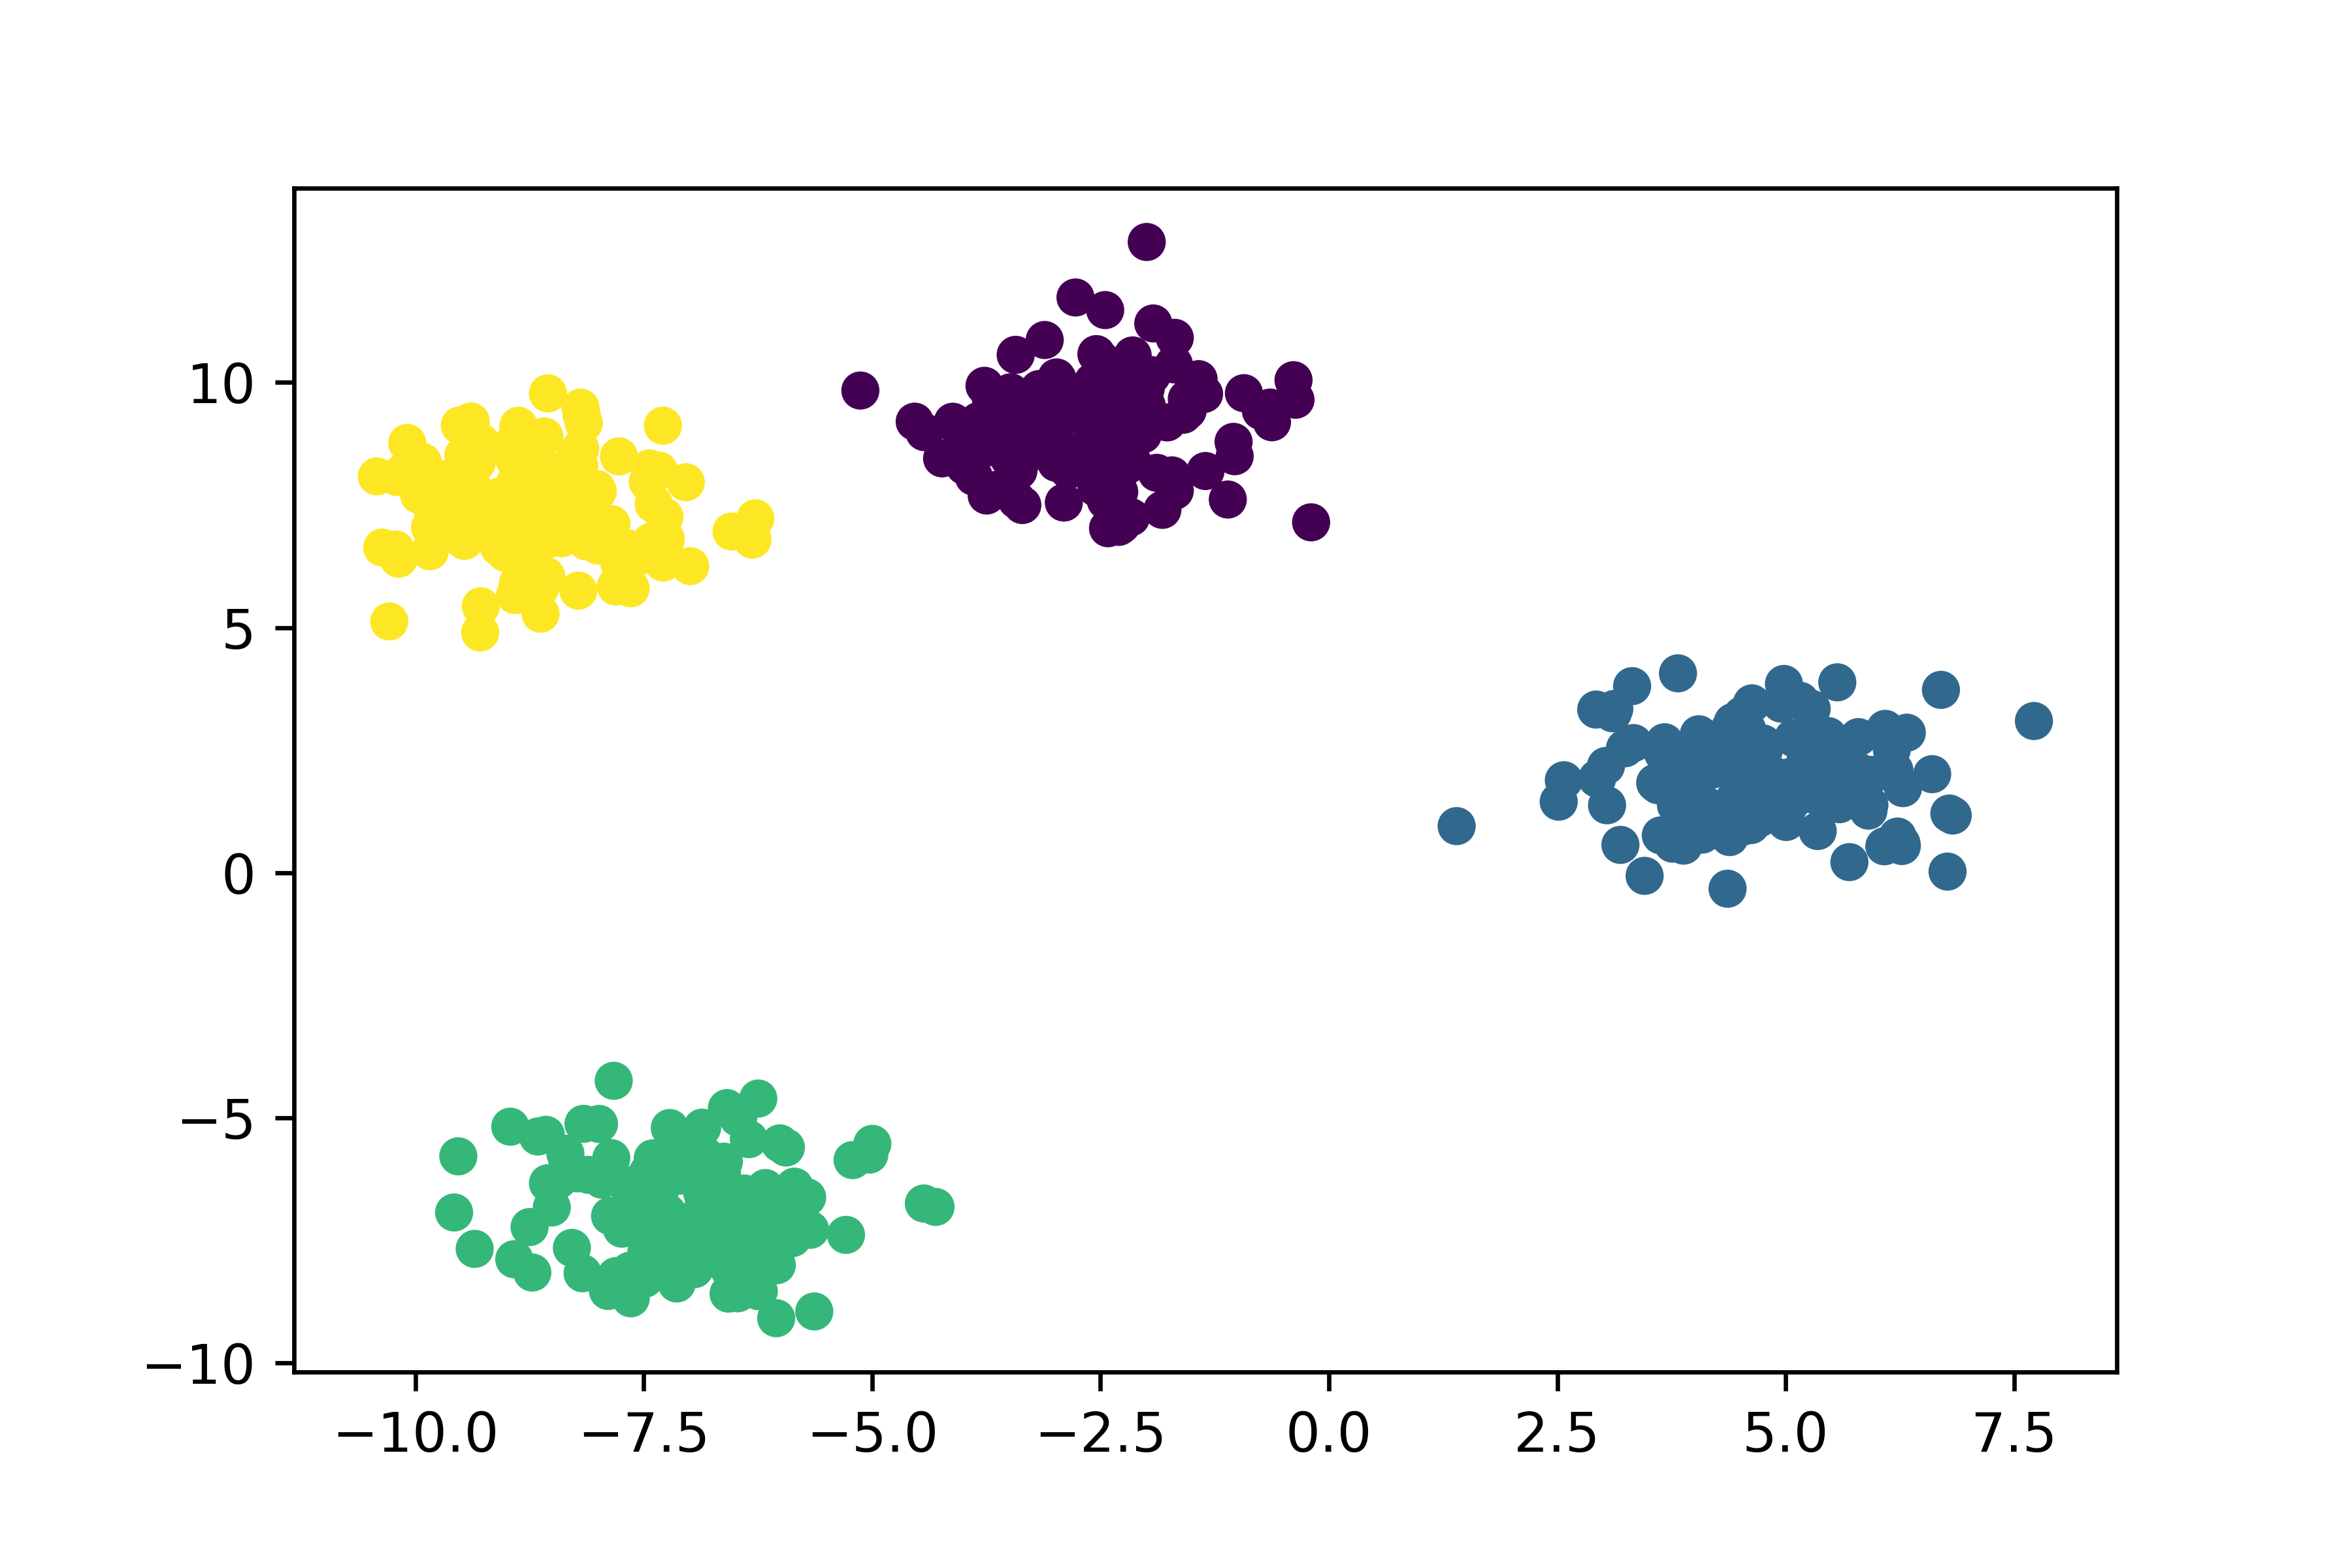
\includegraphics[width=0.55\linewidth]{d1.png}
    \caption{Original Dataset and expected cluster assignments}
\end{figure}
\vspace*{-0.7cm}
\begin{figure}[htbp!]
    \begin{subfigure}{0.33\linewidth}
        \centering
        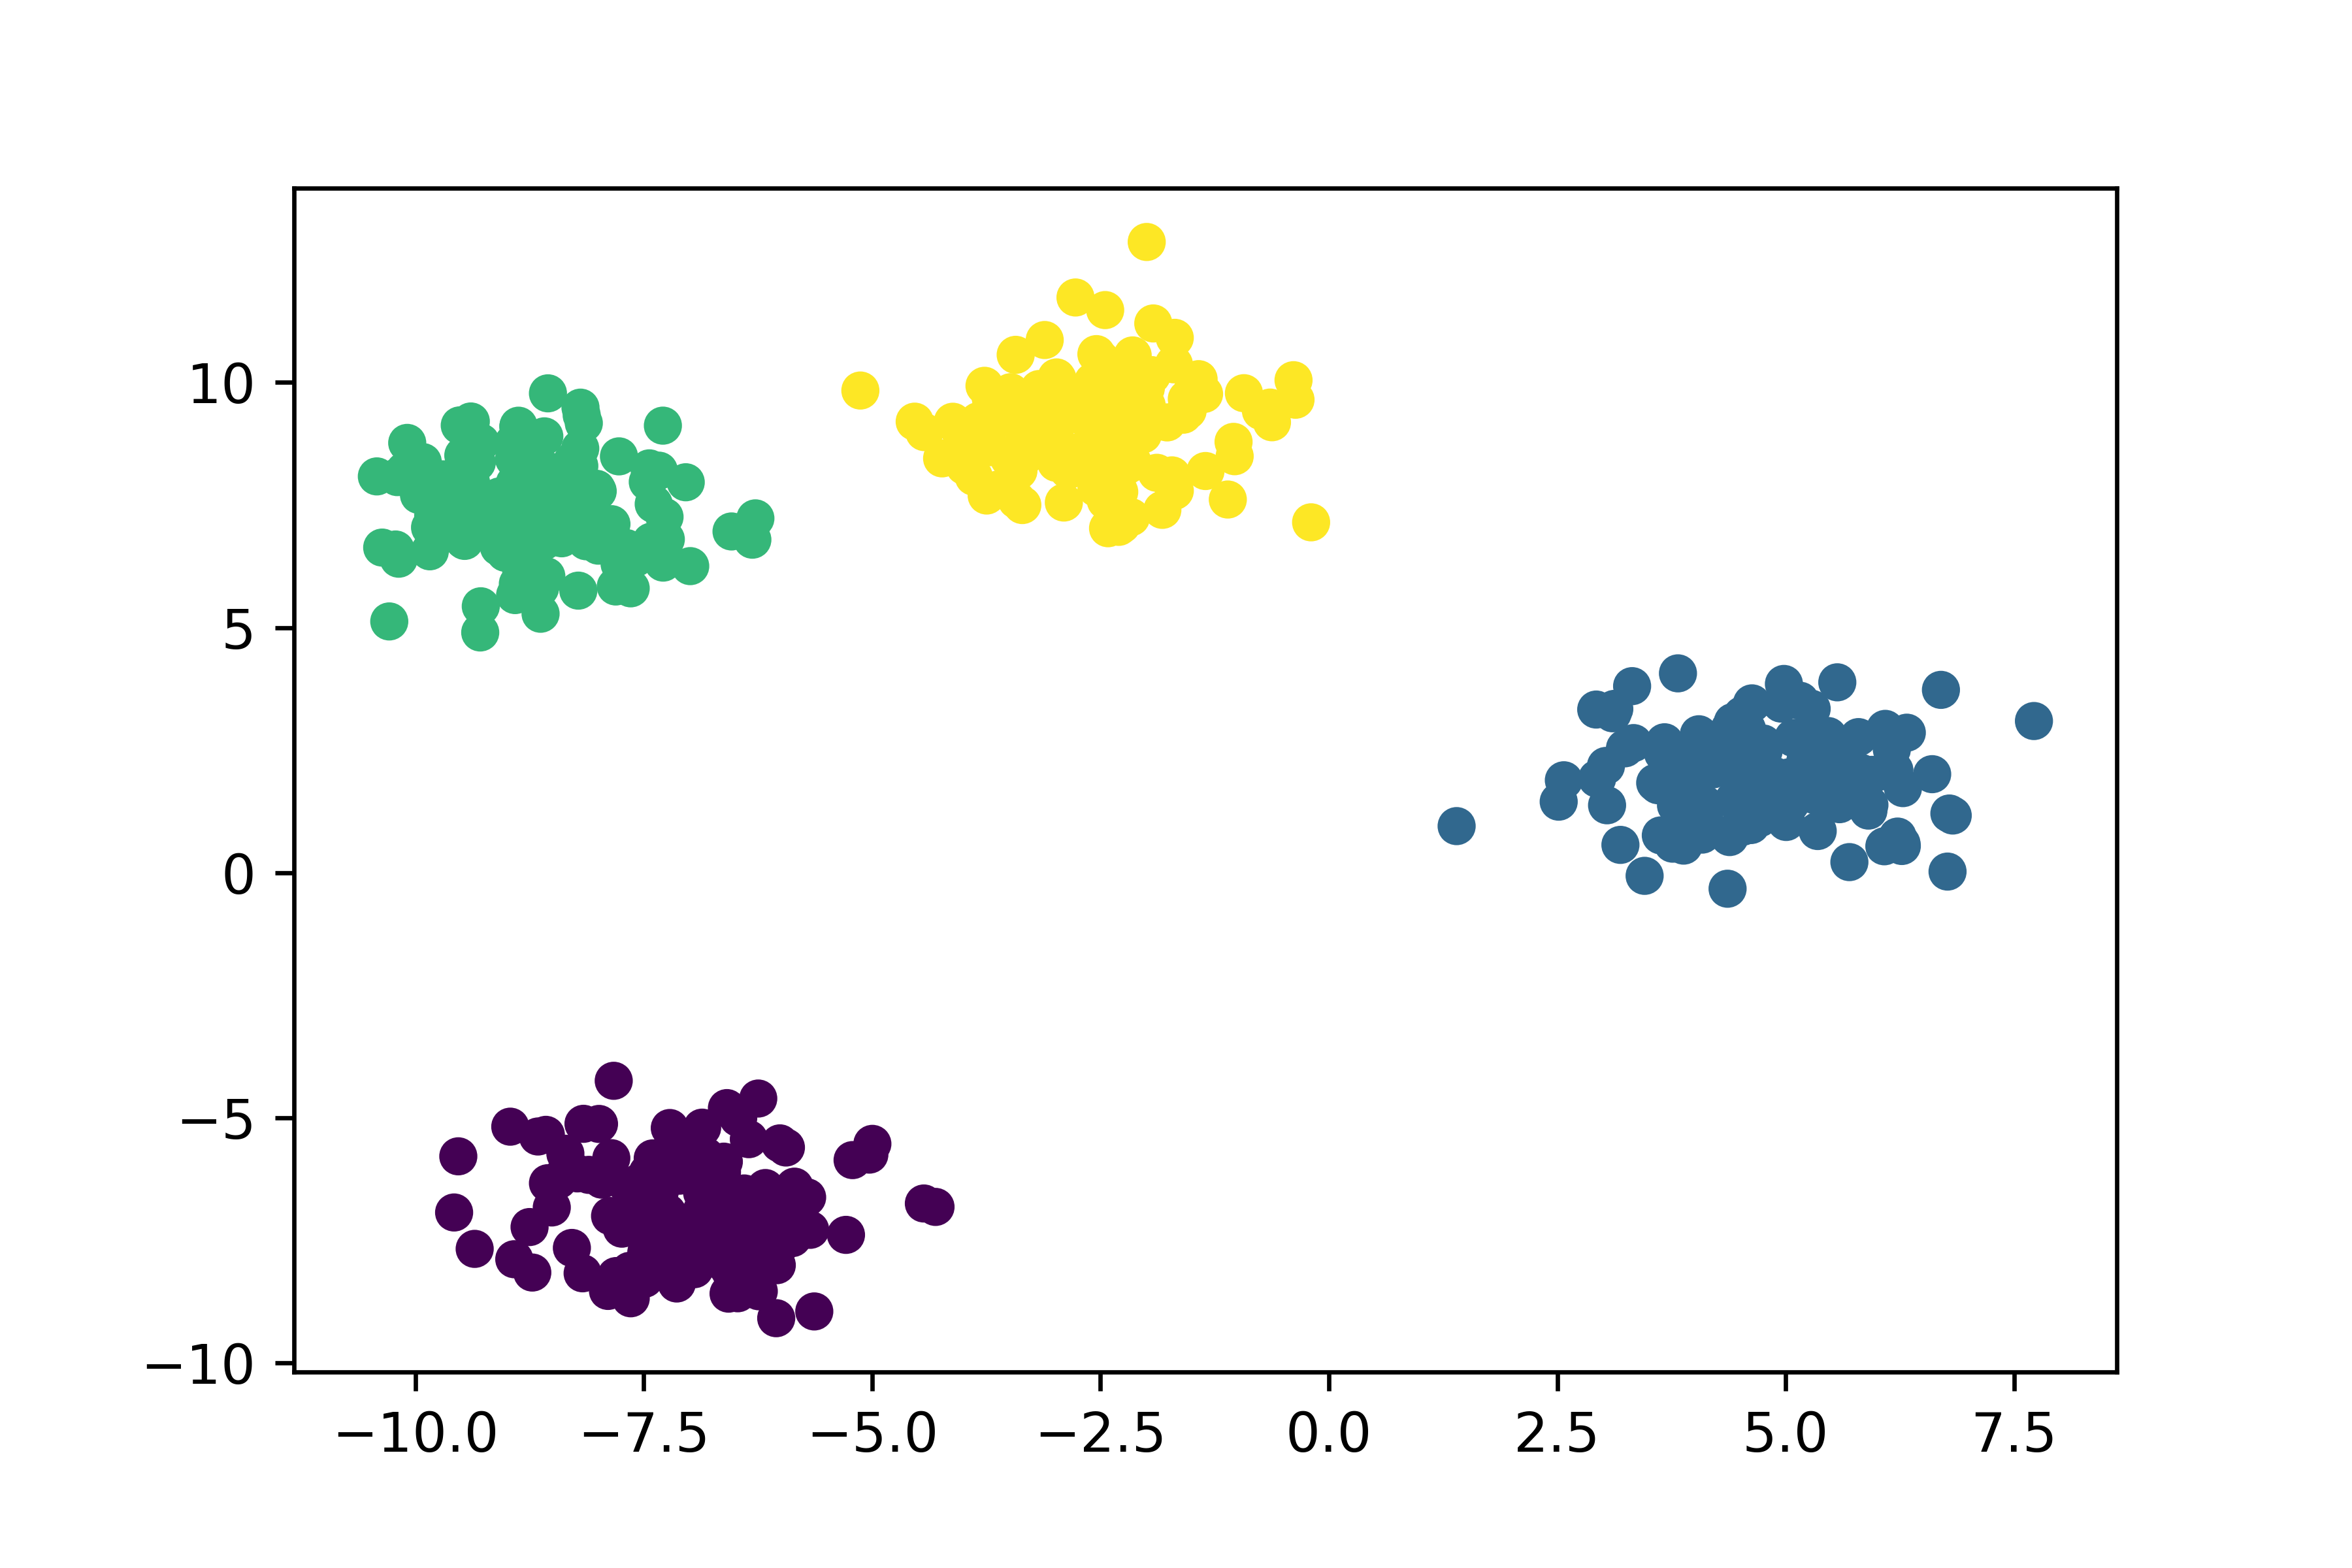
\includegraphics[width=1\linewidth]{d1_123.png}
        \caption{\textbf{SEED=123}}
    \end{subfigure}%
    \begin{subfigure}{0.33\linewidth}
        \centering
        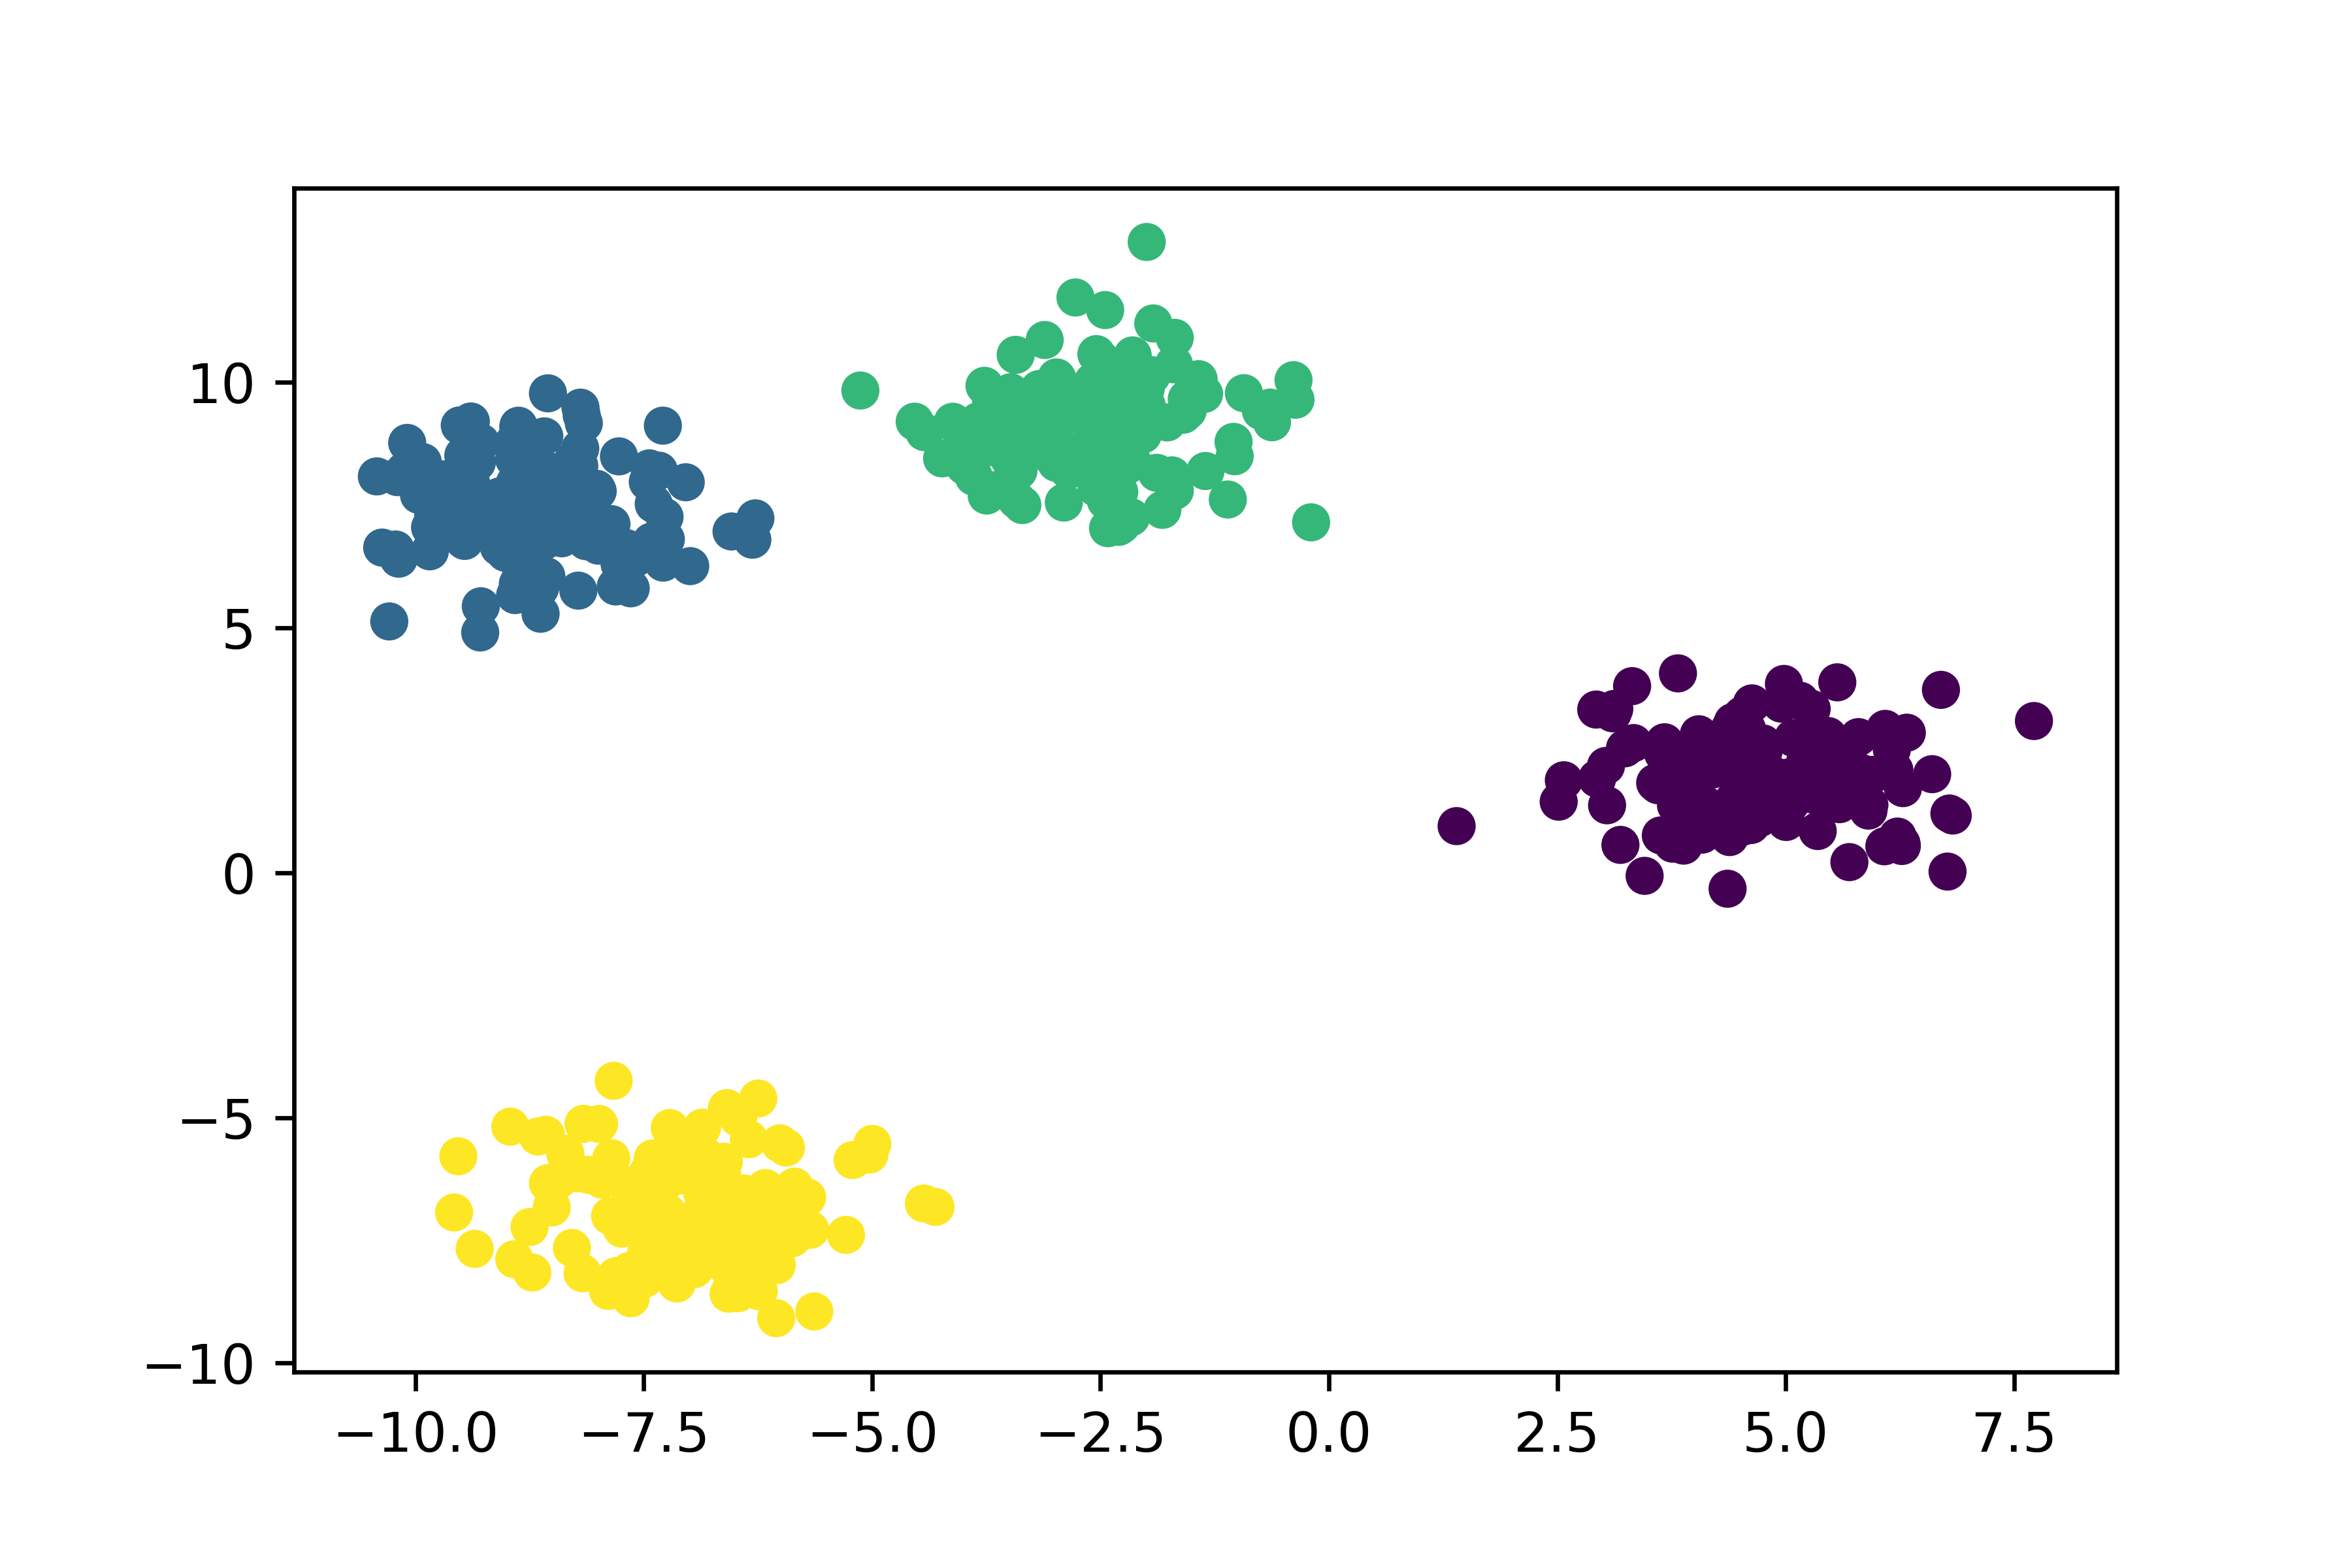
\includegraphics[width=1\linewidth]{d1_53641.png}
        \caption{\textbf{SEED=53641}}
    \end{subfigure}%
    \begin{subfigure}{0.33\linewidth}
        \centering
        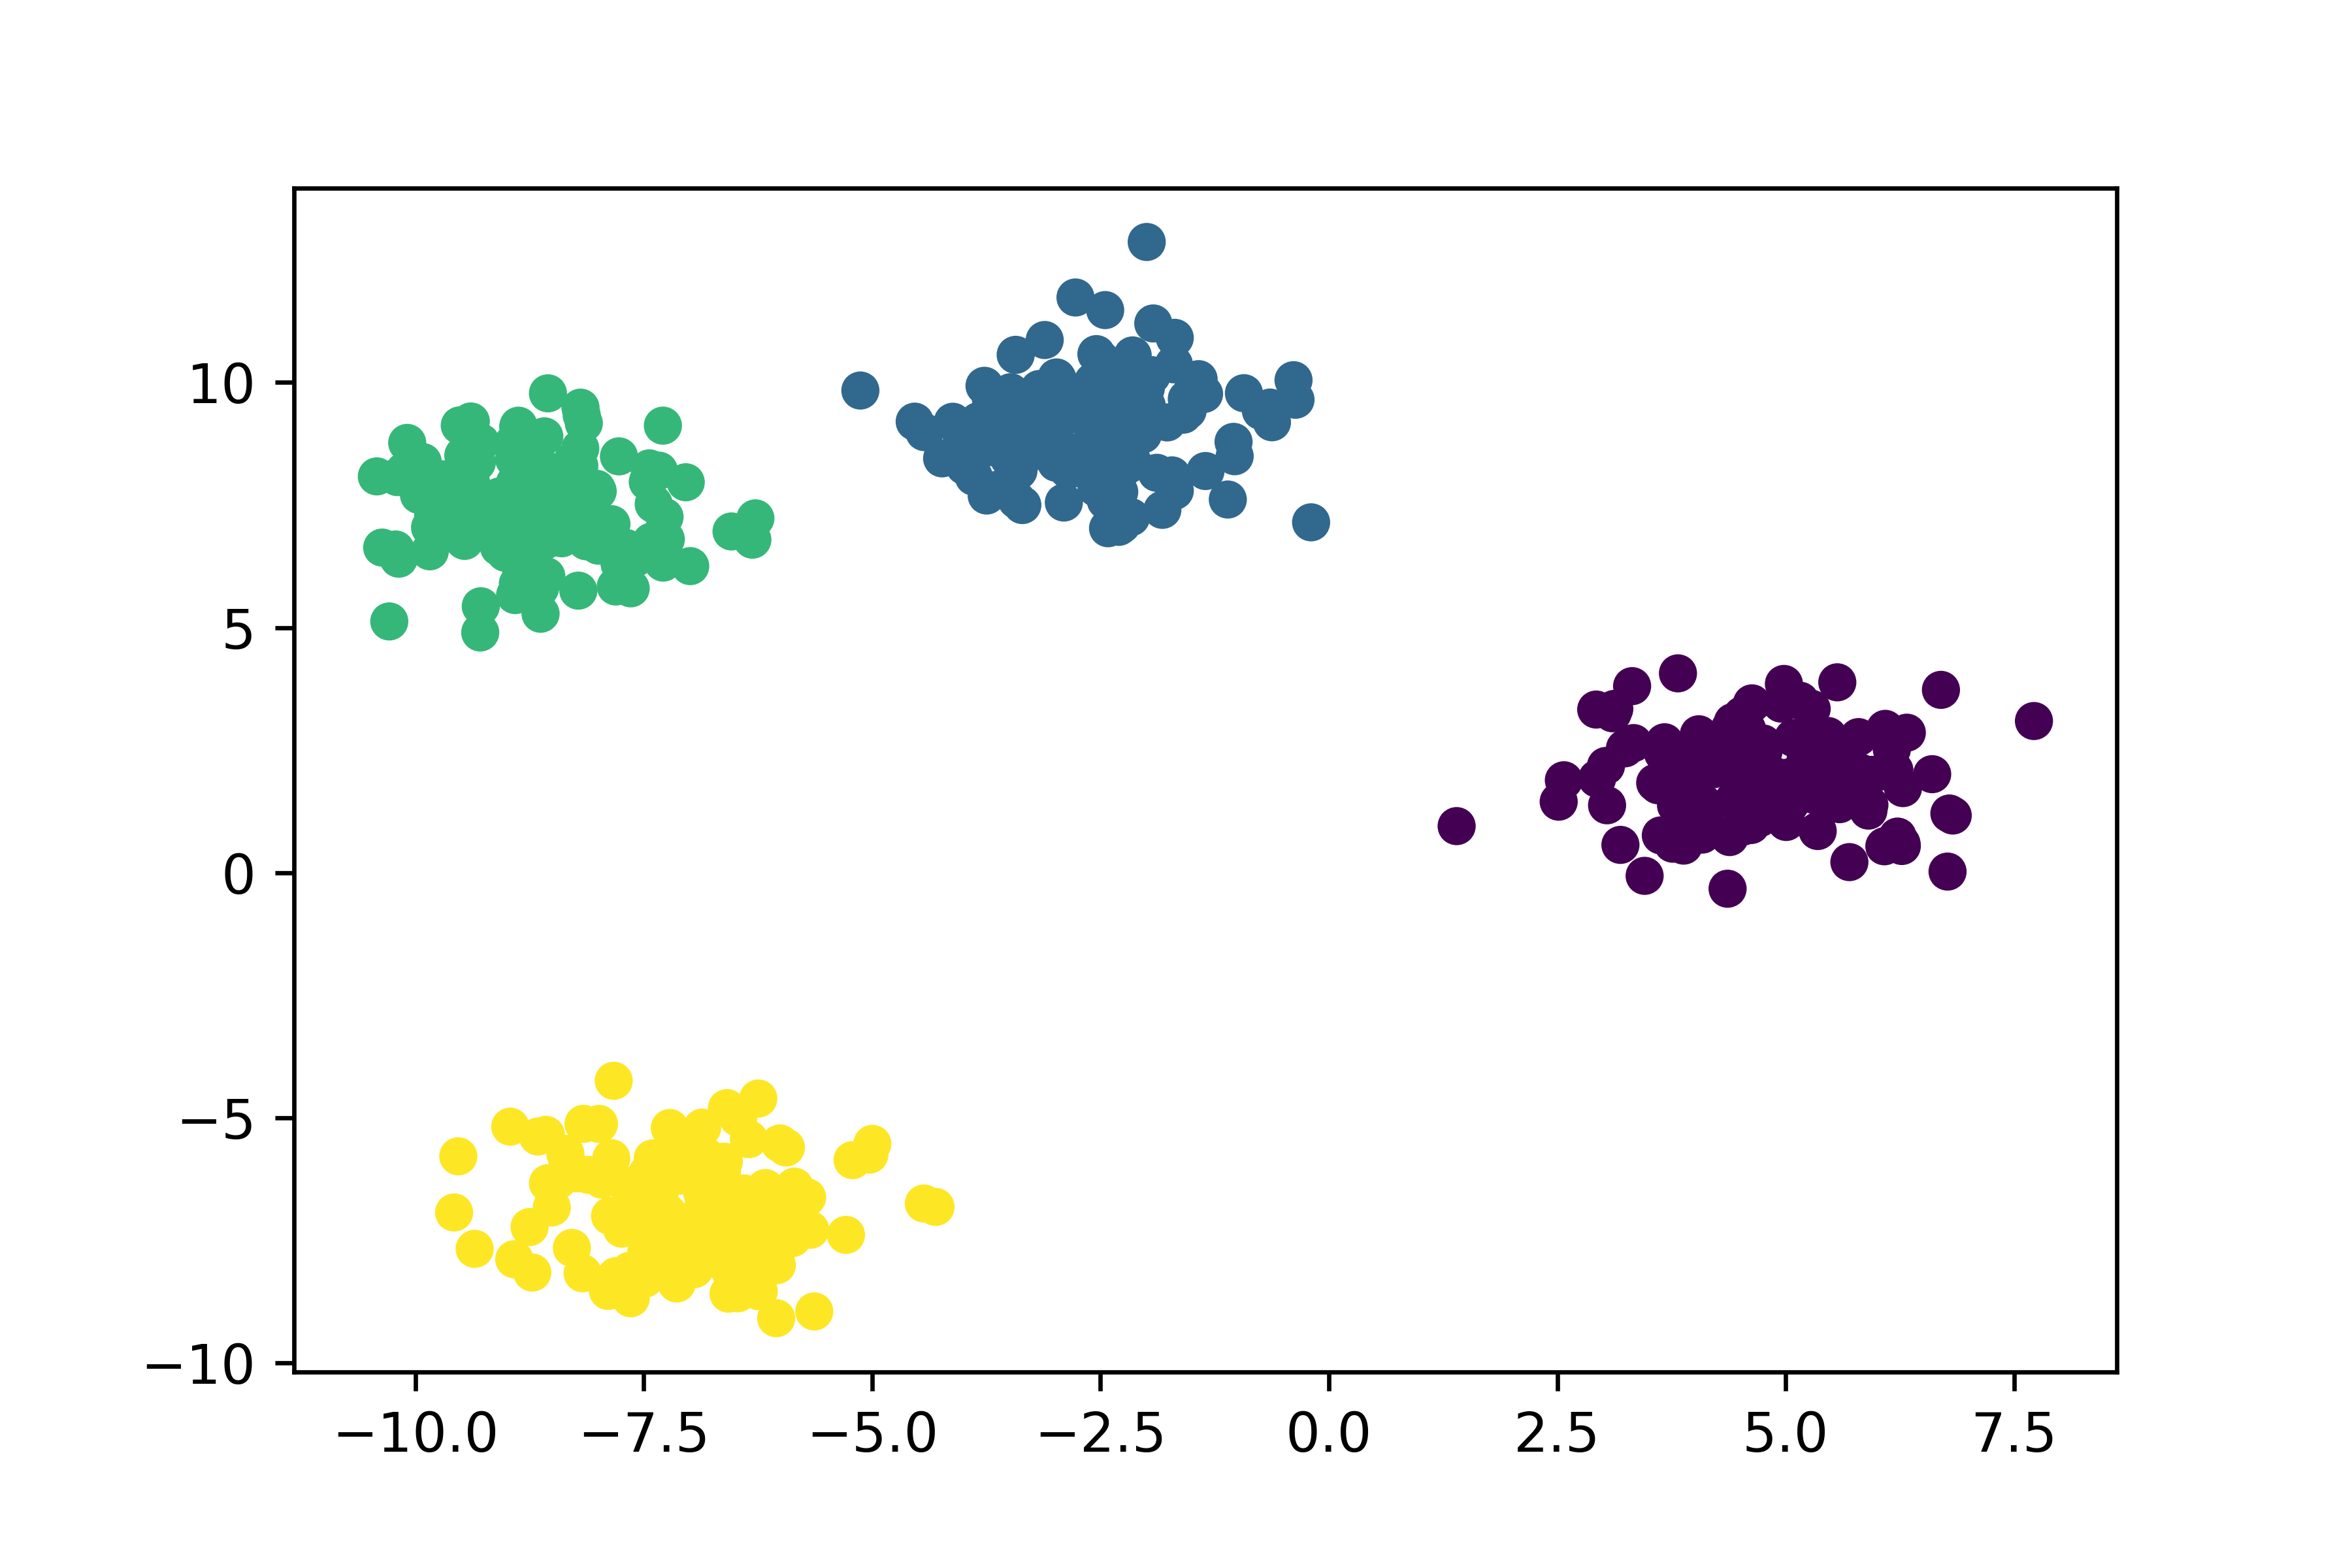
\includegraphics[width=1\linewidth]{d1_87234.png}
        \caption{\textbf{SEED=87234}}
    \end{subfigure}    
\end{figure}

{\Large \textbf{Comments: }} 
\begin{itemize}
    \item For a linearly separable dataset, like the Dataset 1, we find that under good cluster centre initialisations K-MEANS achieves very good results.
    
    \item K-MEANS is highly dependent on the nature of initialisation. If the initialisation is not good, we achieve unintuitive clustering, much because it tries to minimize the plain euclidean distance based on the cluster centre initialisation and gets stuck in a local minima.
    
    \item K-MEANS is not suited for the type of clustering expected in Dataset 2 or 3. We can observe that K-MEANS is not suited for non-convex clustering. Dataset 2 and 3 are not linearly separable. 
    
    \item There are no ideal ``cluster centres'' for dataset 2 and 3 which will return the type of clusters we want. K-MEANS is not checking the pairwise closeness of cluster points. Its rather allotting points to the nearest cluster centre. To this end the type of clusters we receive with K-MEANS is totally expected. The clusters we receive do minimize the overall euclidean distance from their allotted cluster centres.
\end{itemize}

{\large \textbf{DATA 2}}%
\vspace*{-1cm}
\begin{figure}[H]
    \centering
    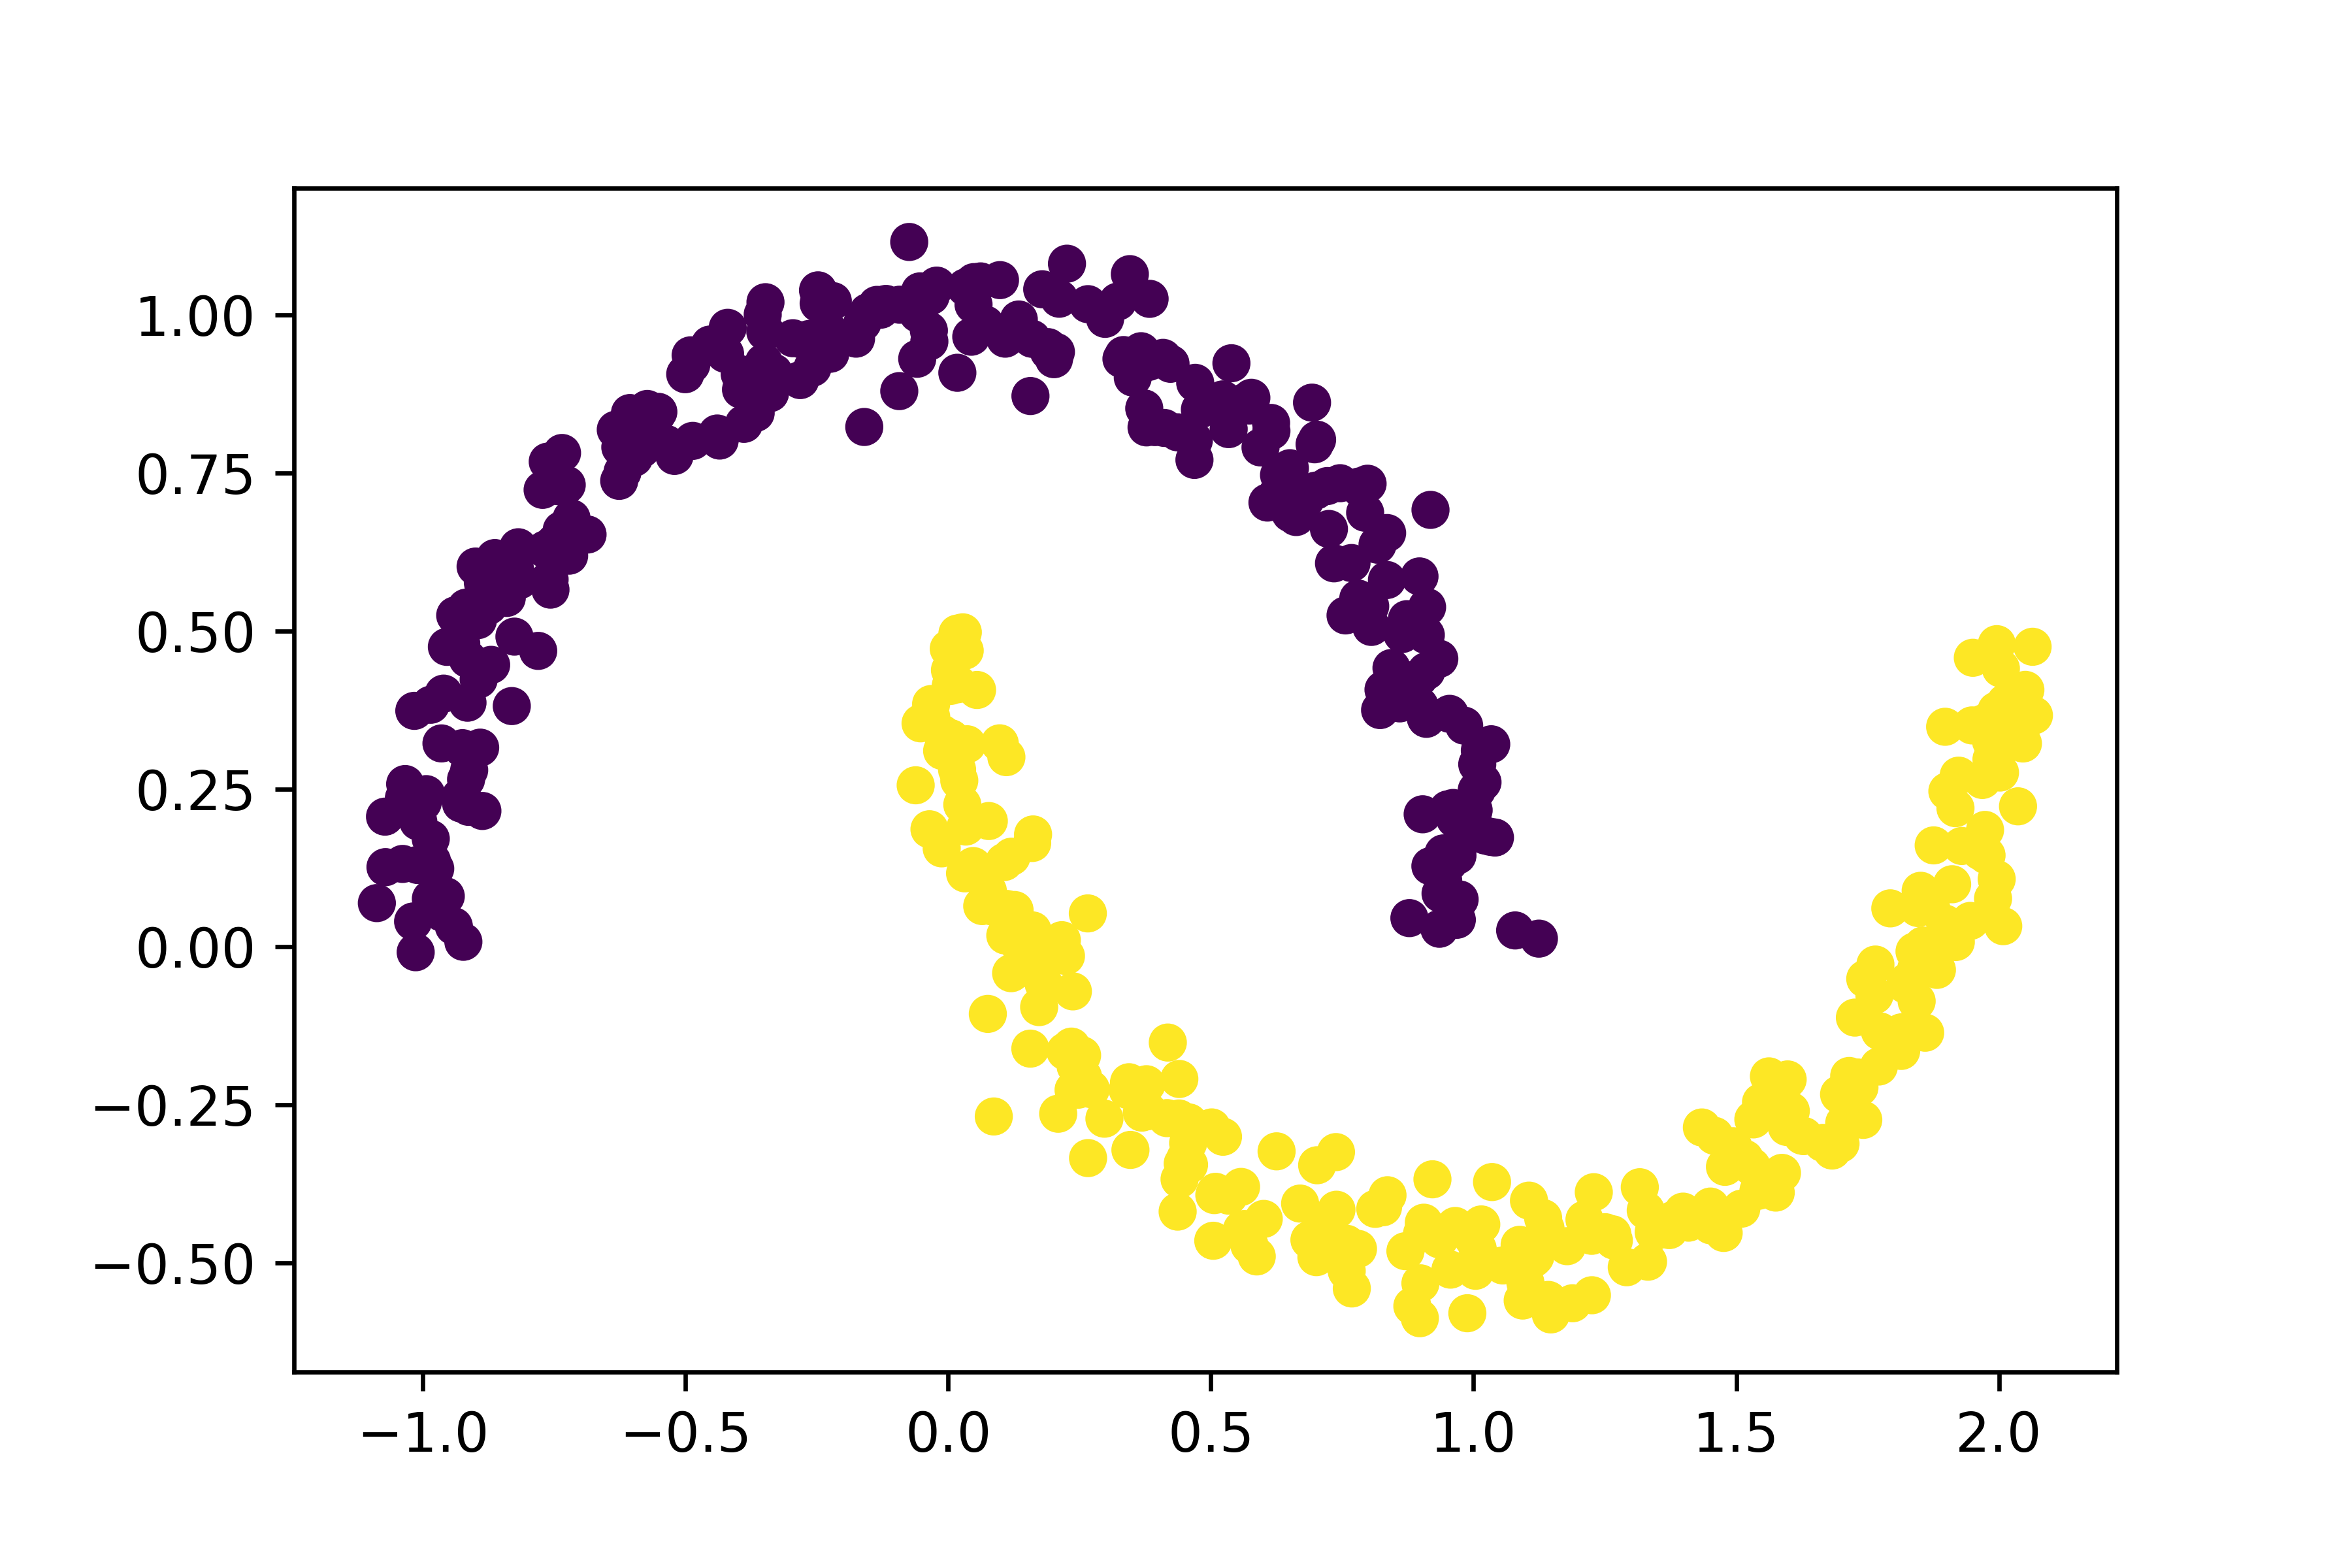
\includegraphics[width=0.55\linewidth]{d2.png}
    \caption{Original Dataset and expected cluster assignments}
\end{figure}%
\vspace*{-0.7cm}
\begin{figure}[H]
    \begin{subfigure}{0.33\linewidth}
        \centering
        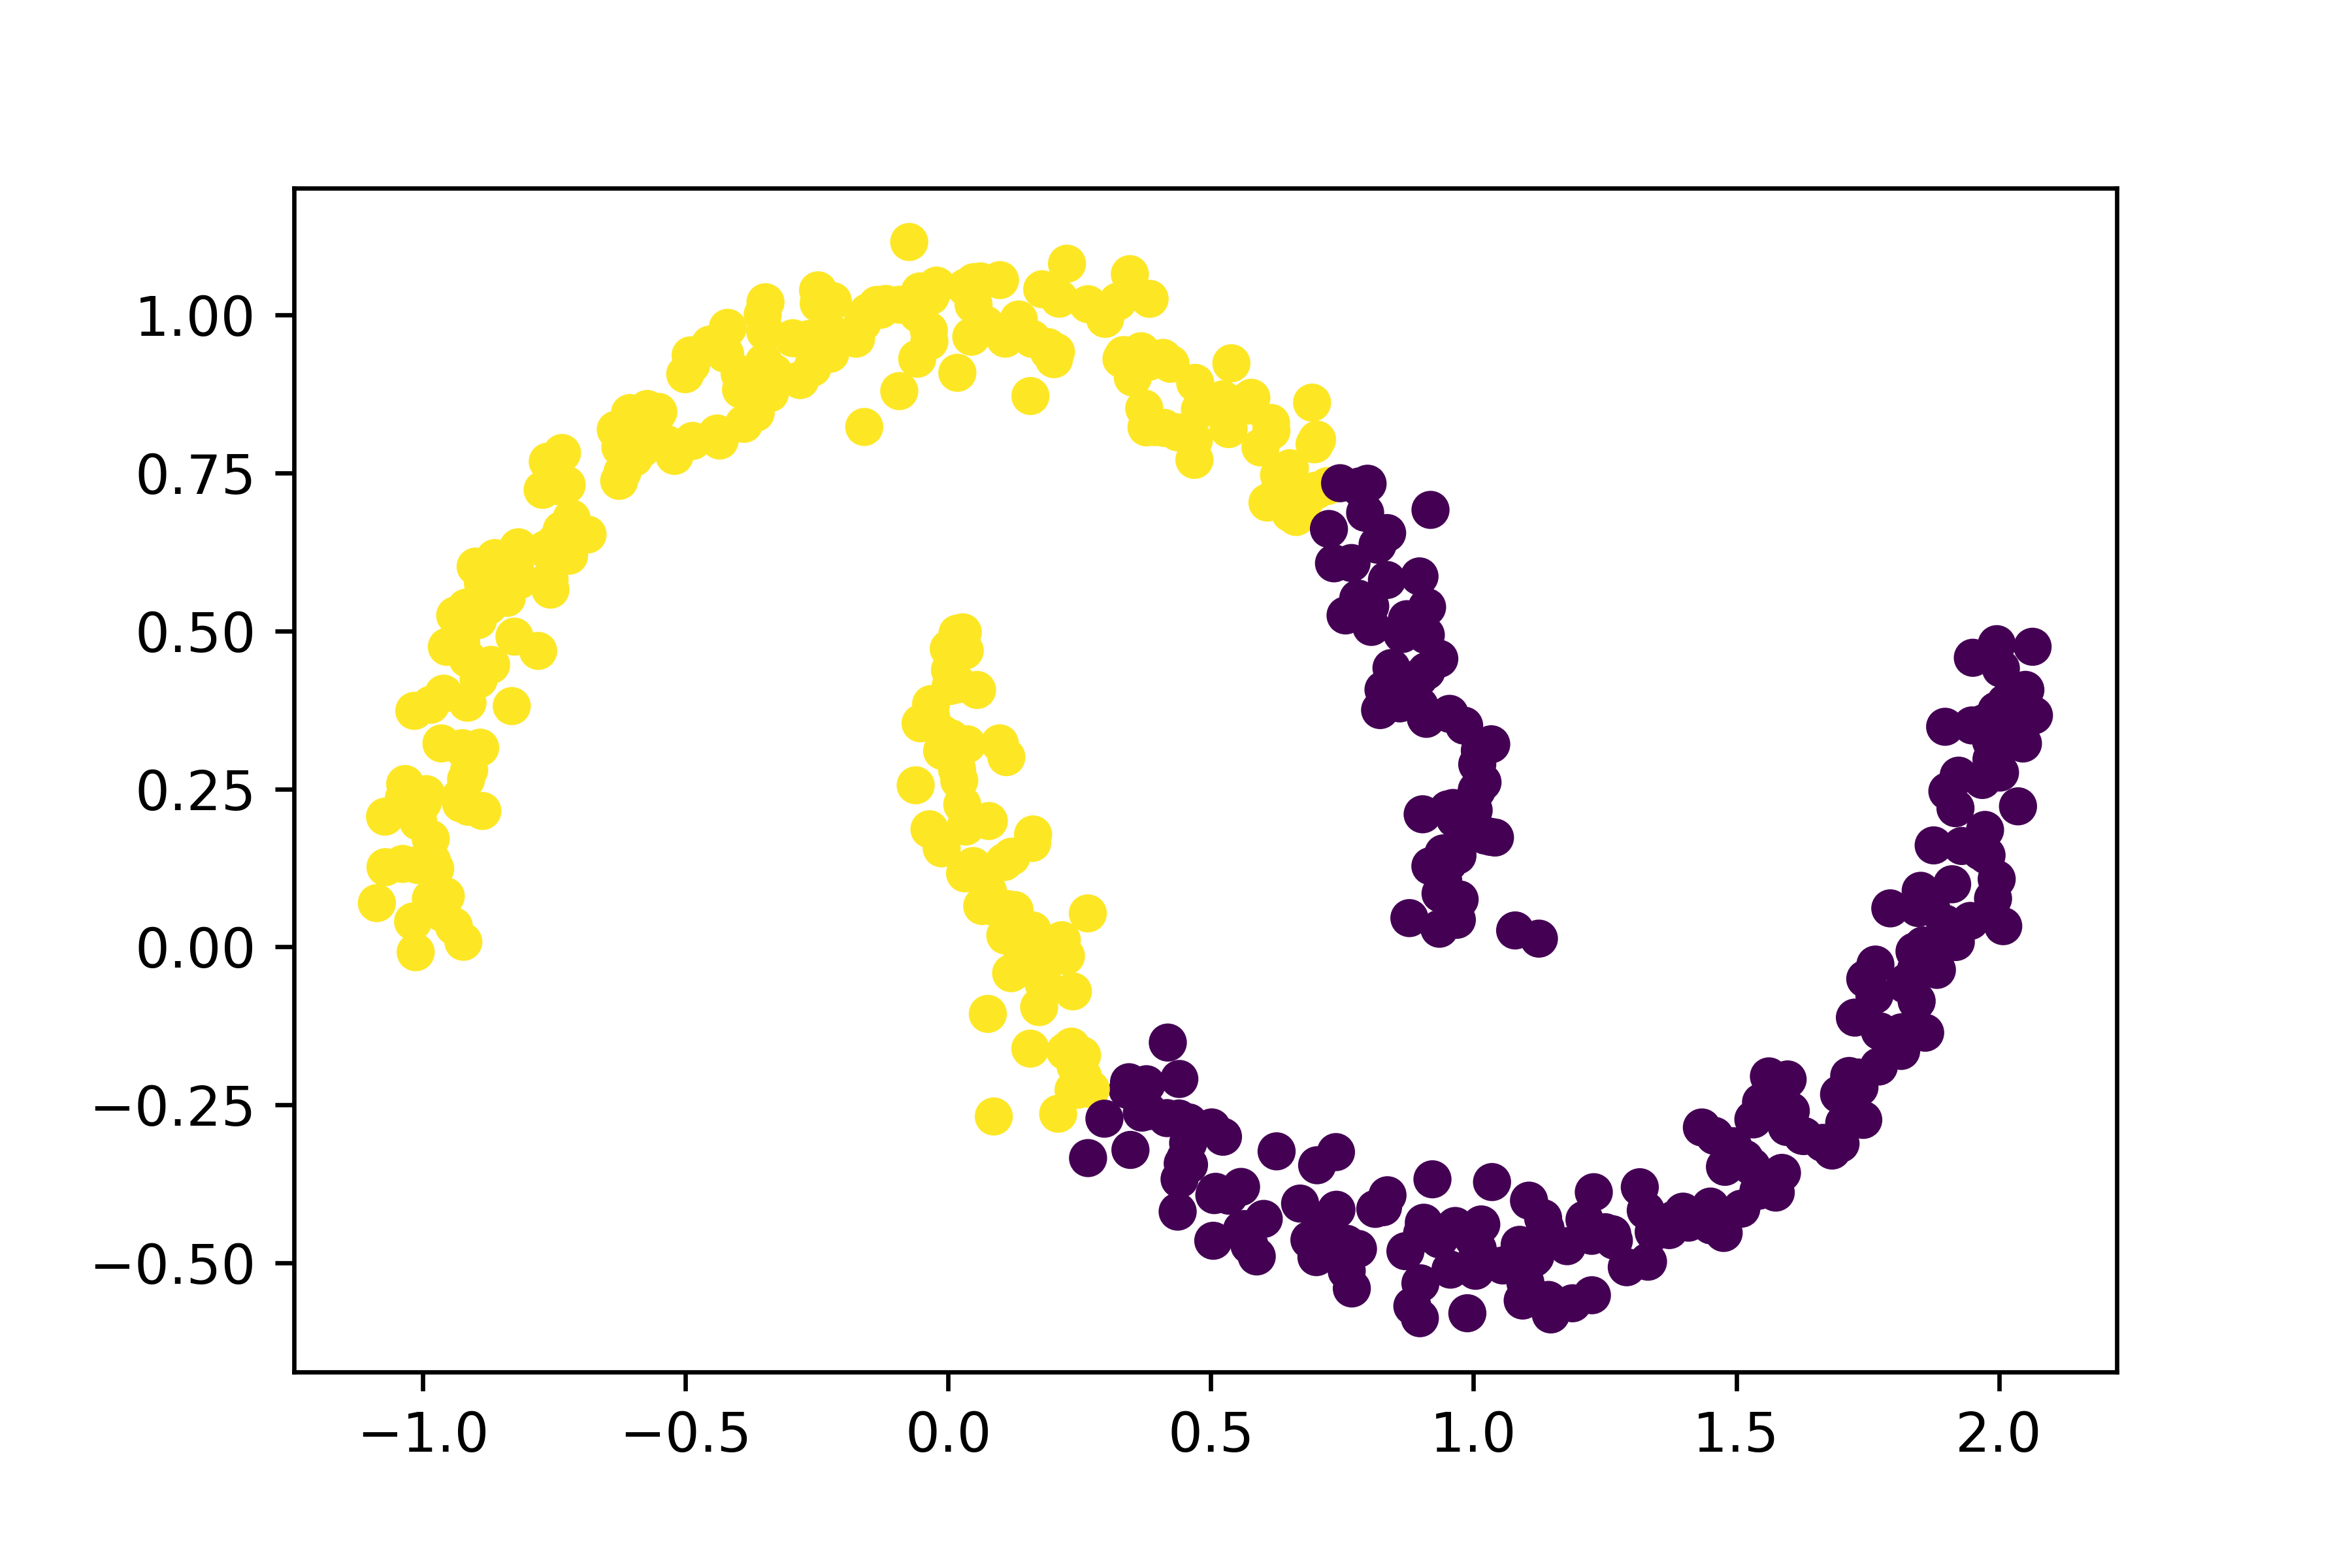
\includegraphics[width=1\linewidth]{d2_123.png}
        \caption{\textbf{SEED=123}}
    \end{subfigure}%
    \begin{subfigure}{0.33\linewidth}
        \centering
        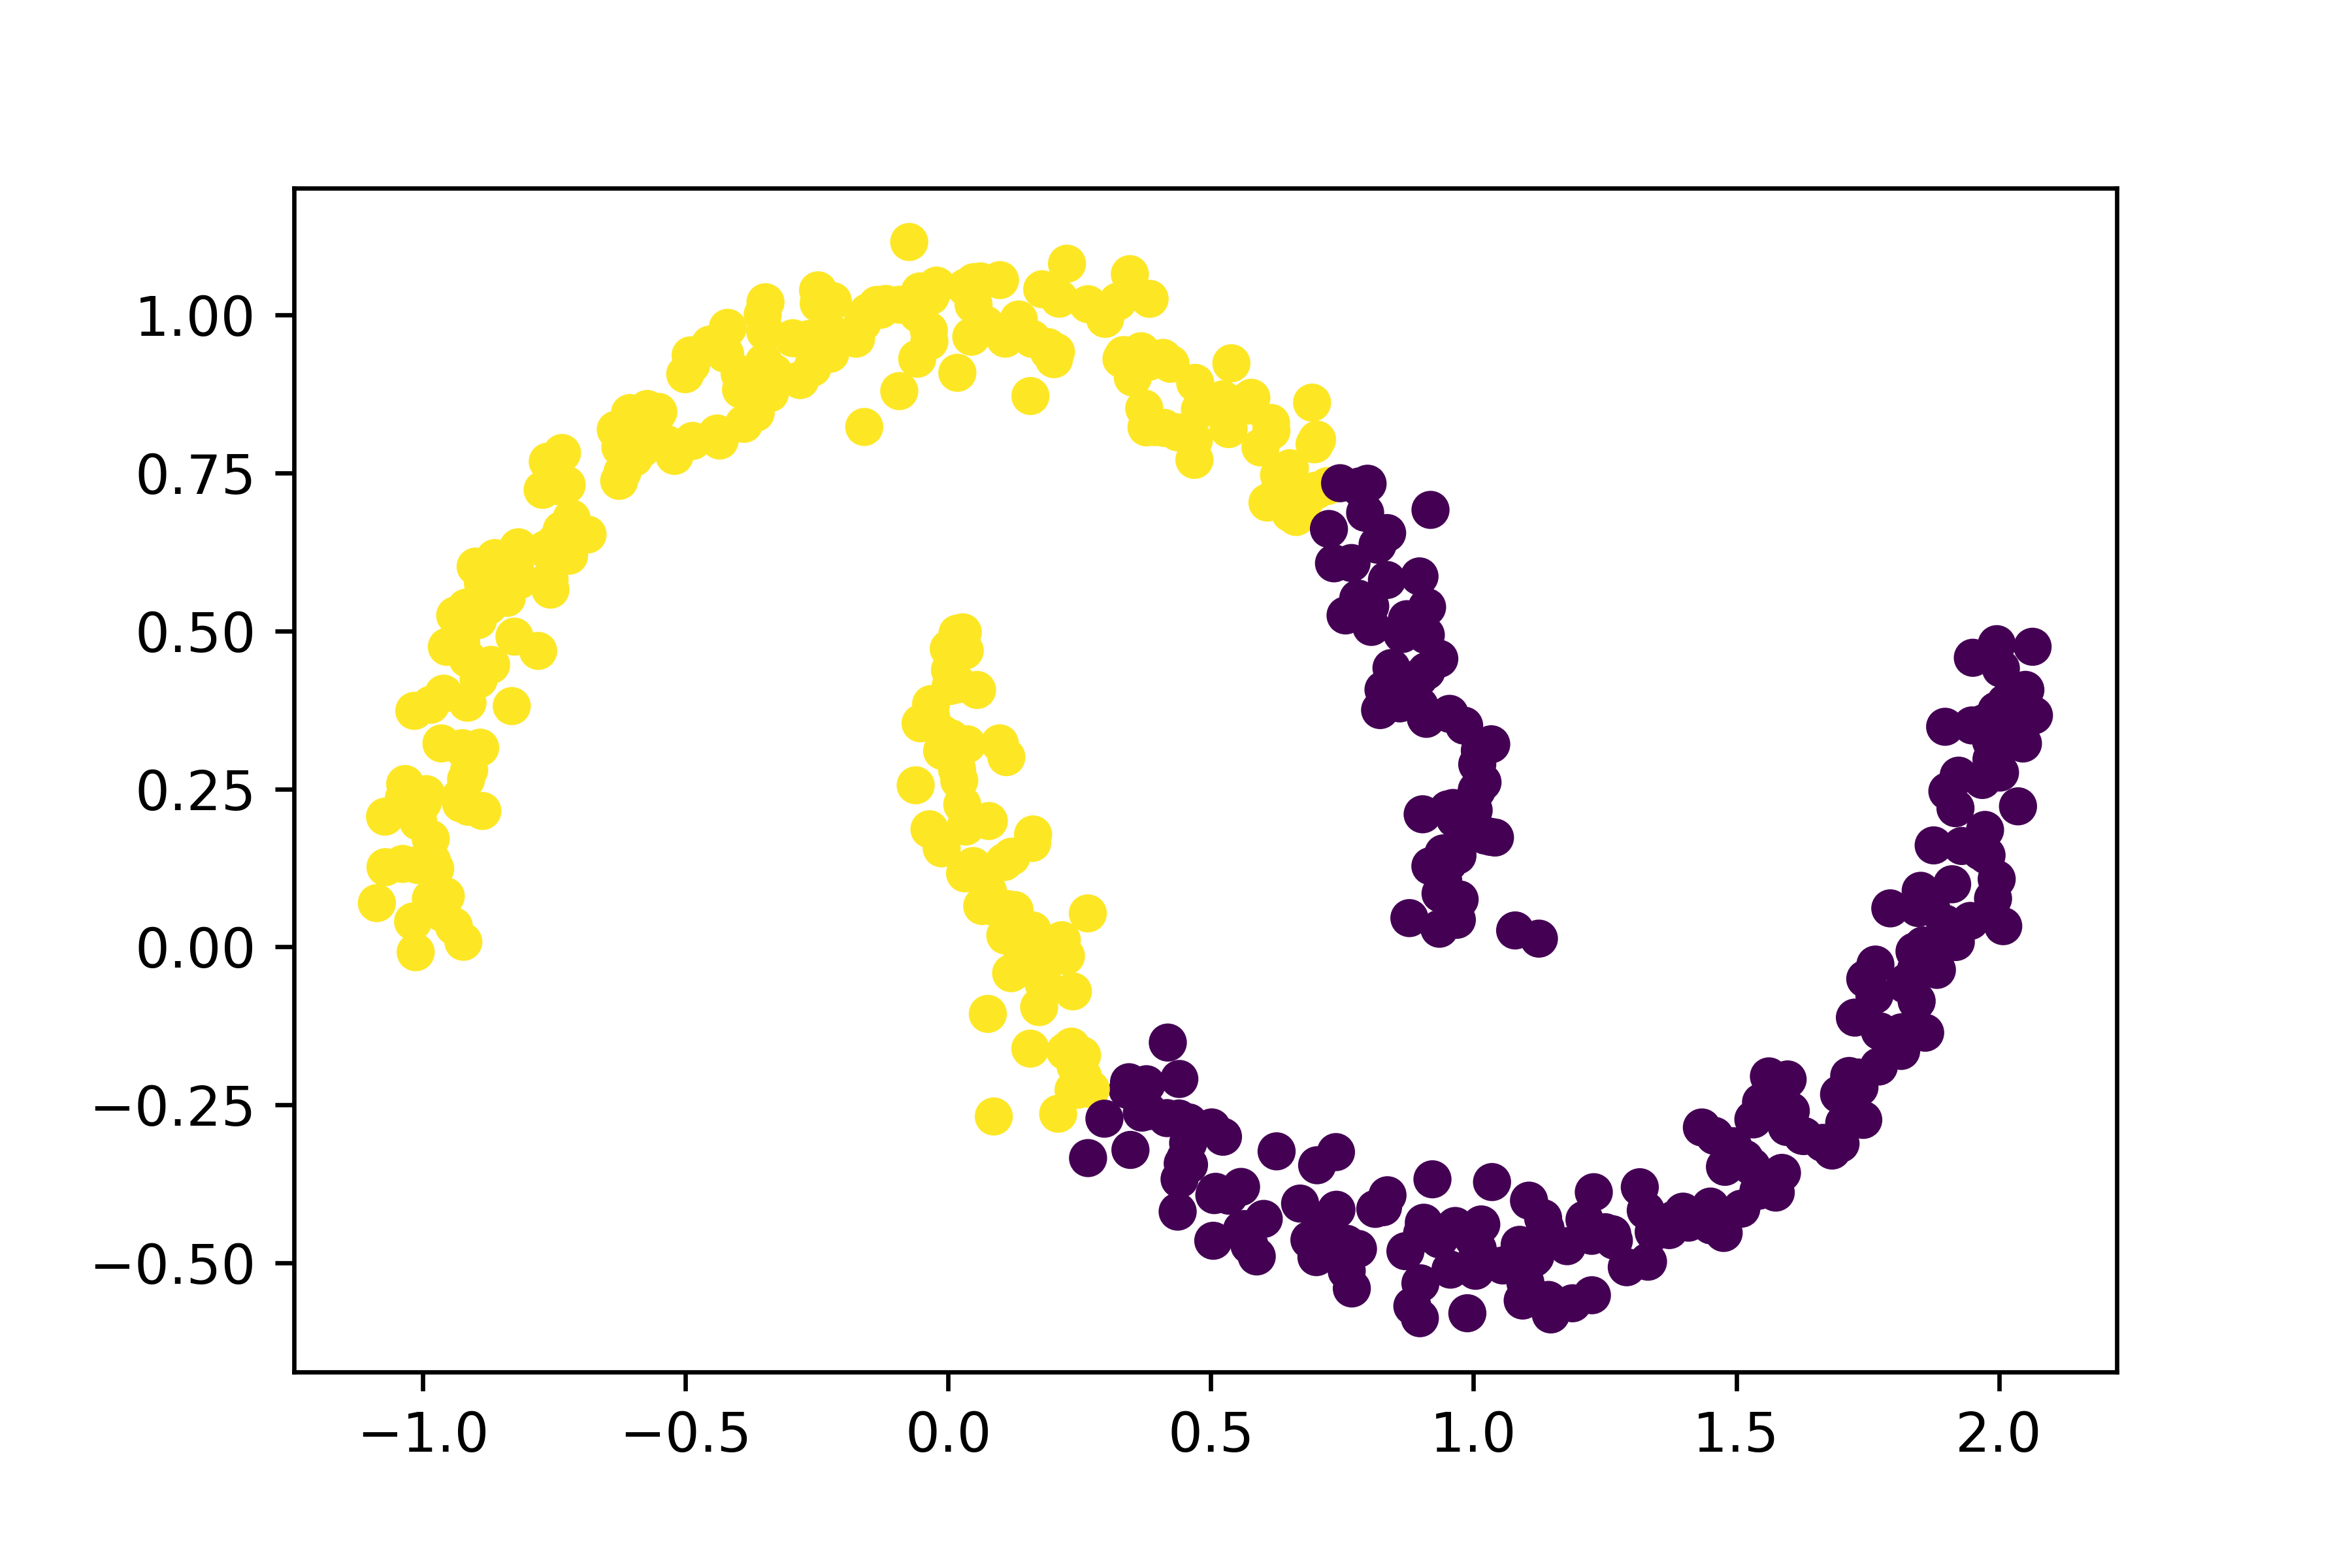
\includegraphics[width=1\linewidth]{d2_53641.png}
        \caption{\textbf{SEED=53641}}
    \end{subfigure}%
    \begin{subfigure}{0.33\linewidth}
        \centering
        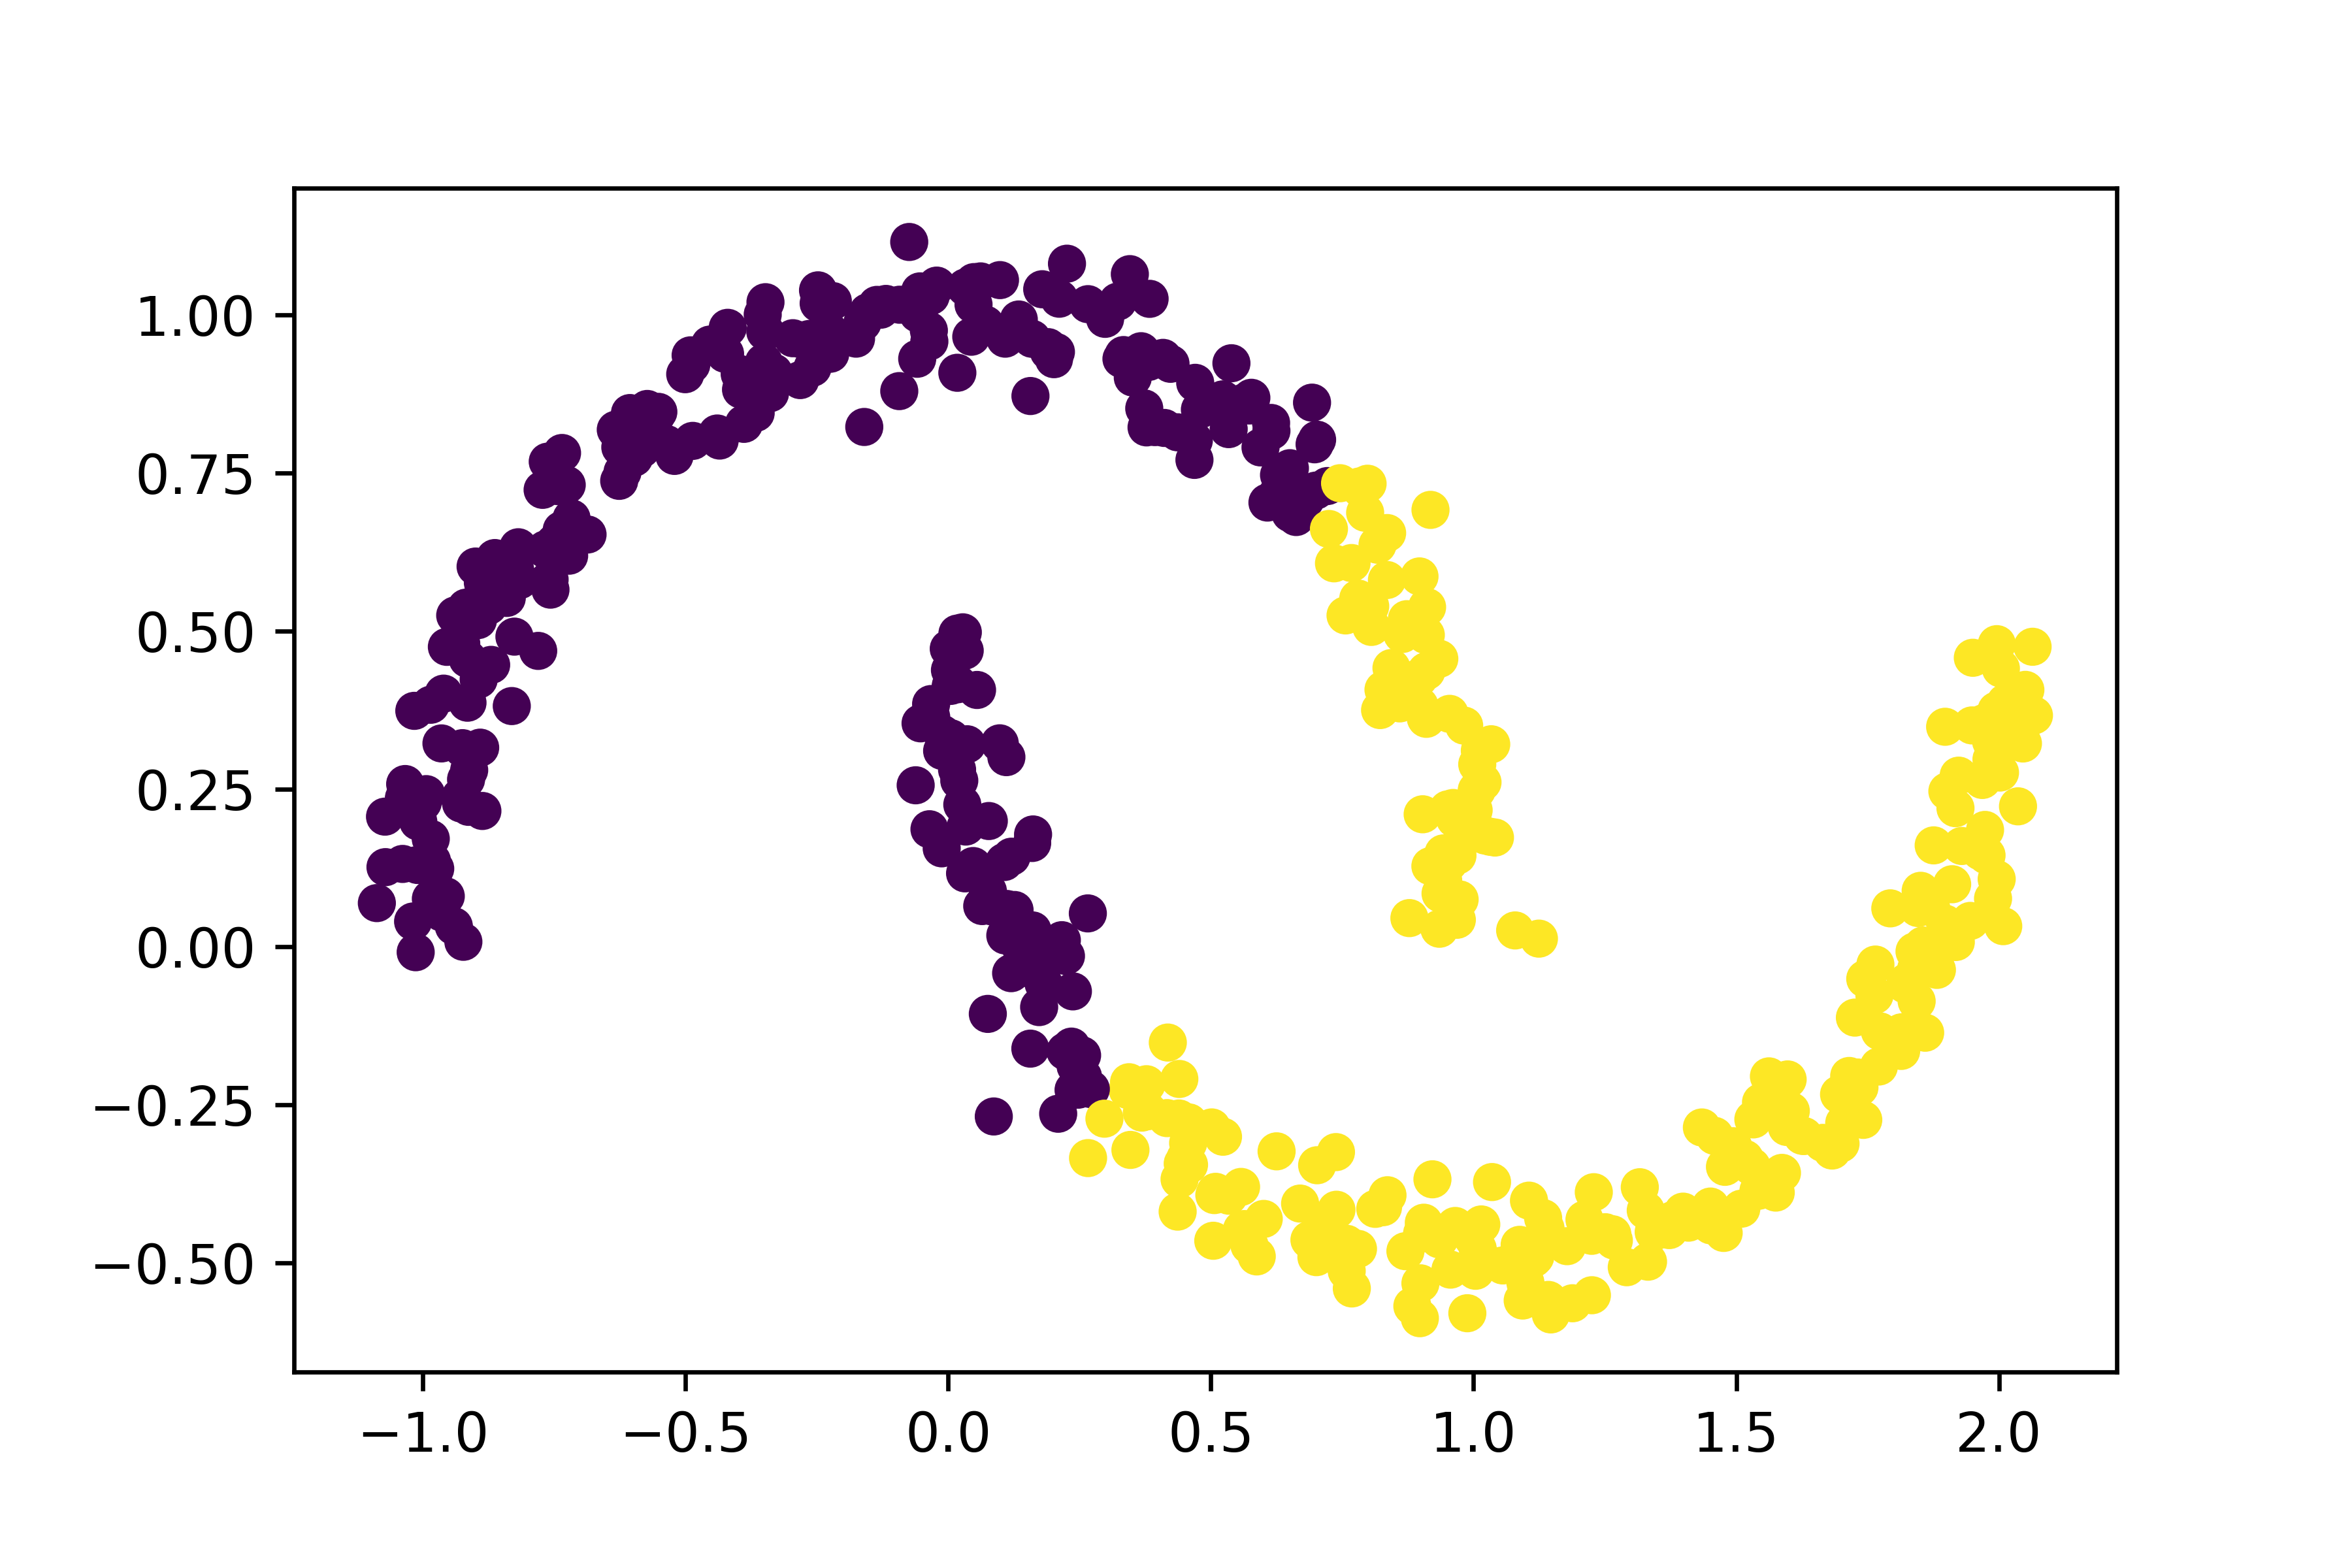
\includegraphics[width=1\linewidth]{d2_87234.png}
        \caption{\textbf{SEED=87234}}
    \end{subfigure}    
\end{figure}%
{\large \textbf{DATA 3}}%
\vspace*{-1cm}
\begin{figure}[H]
    \centering
    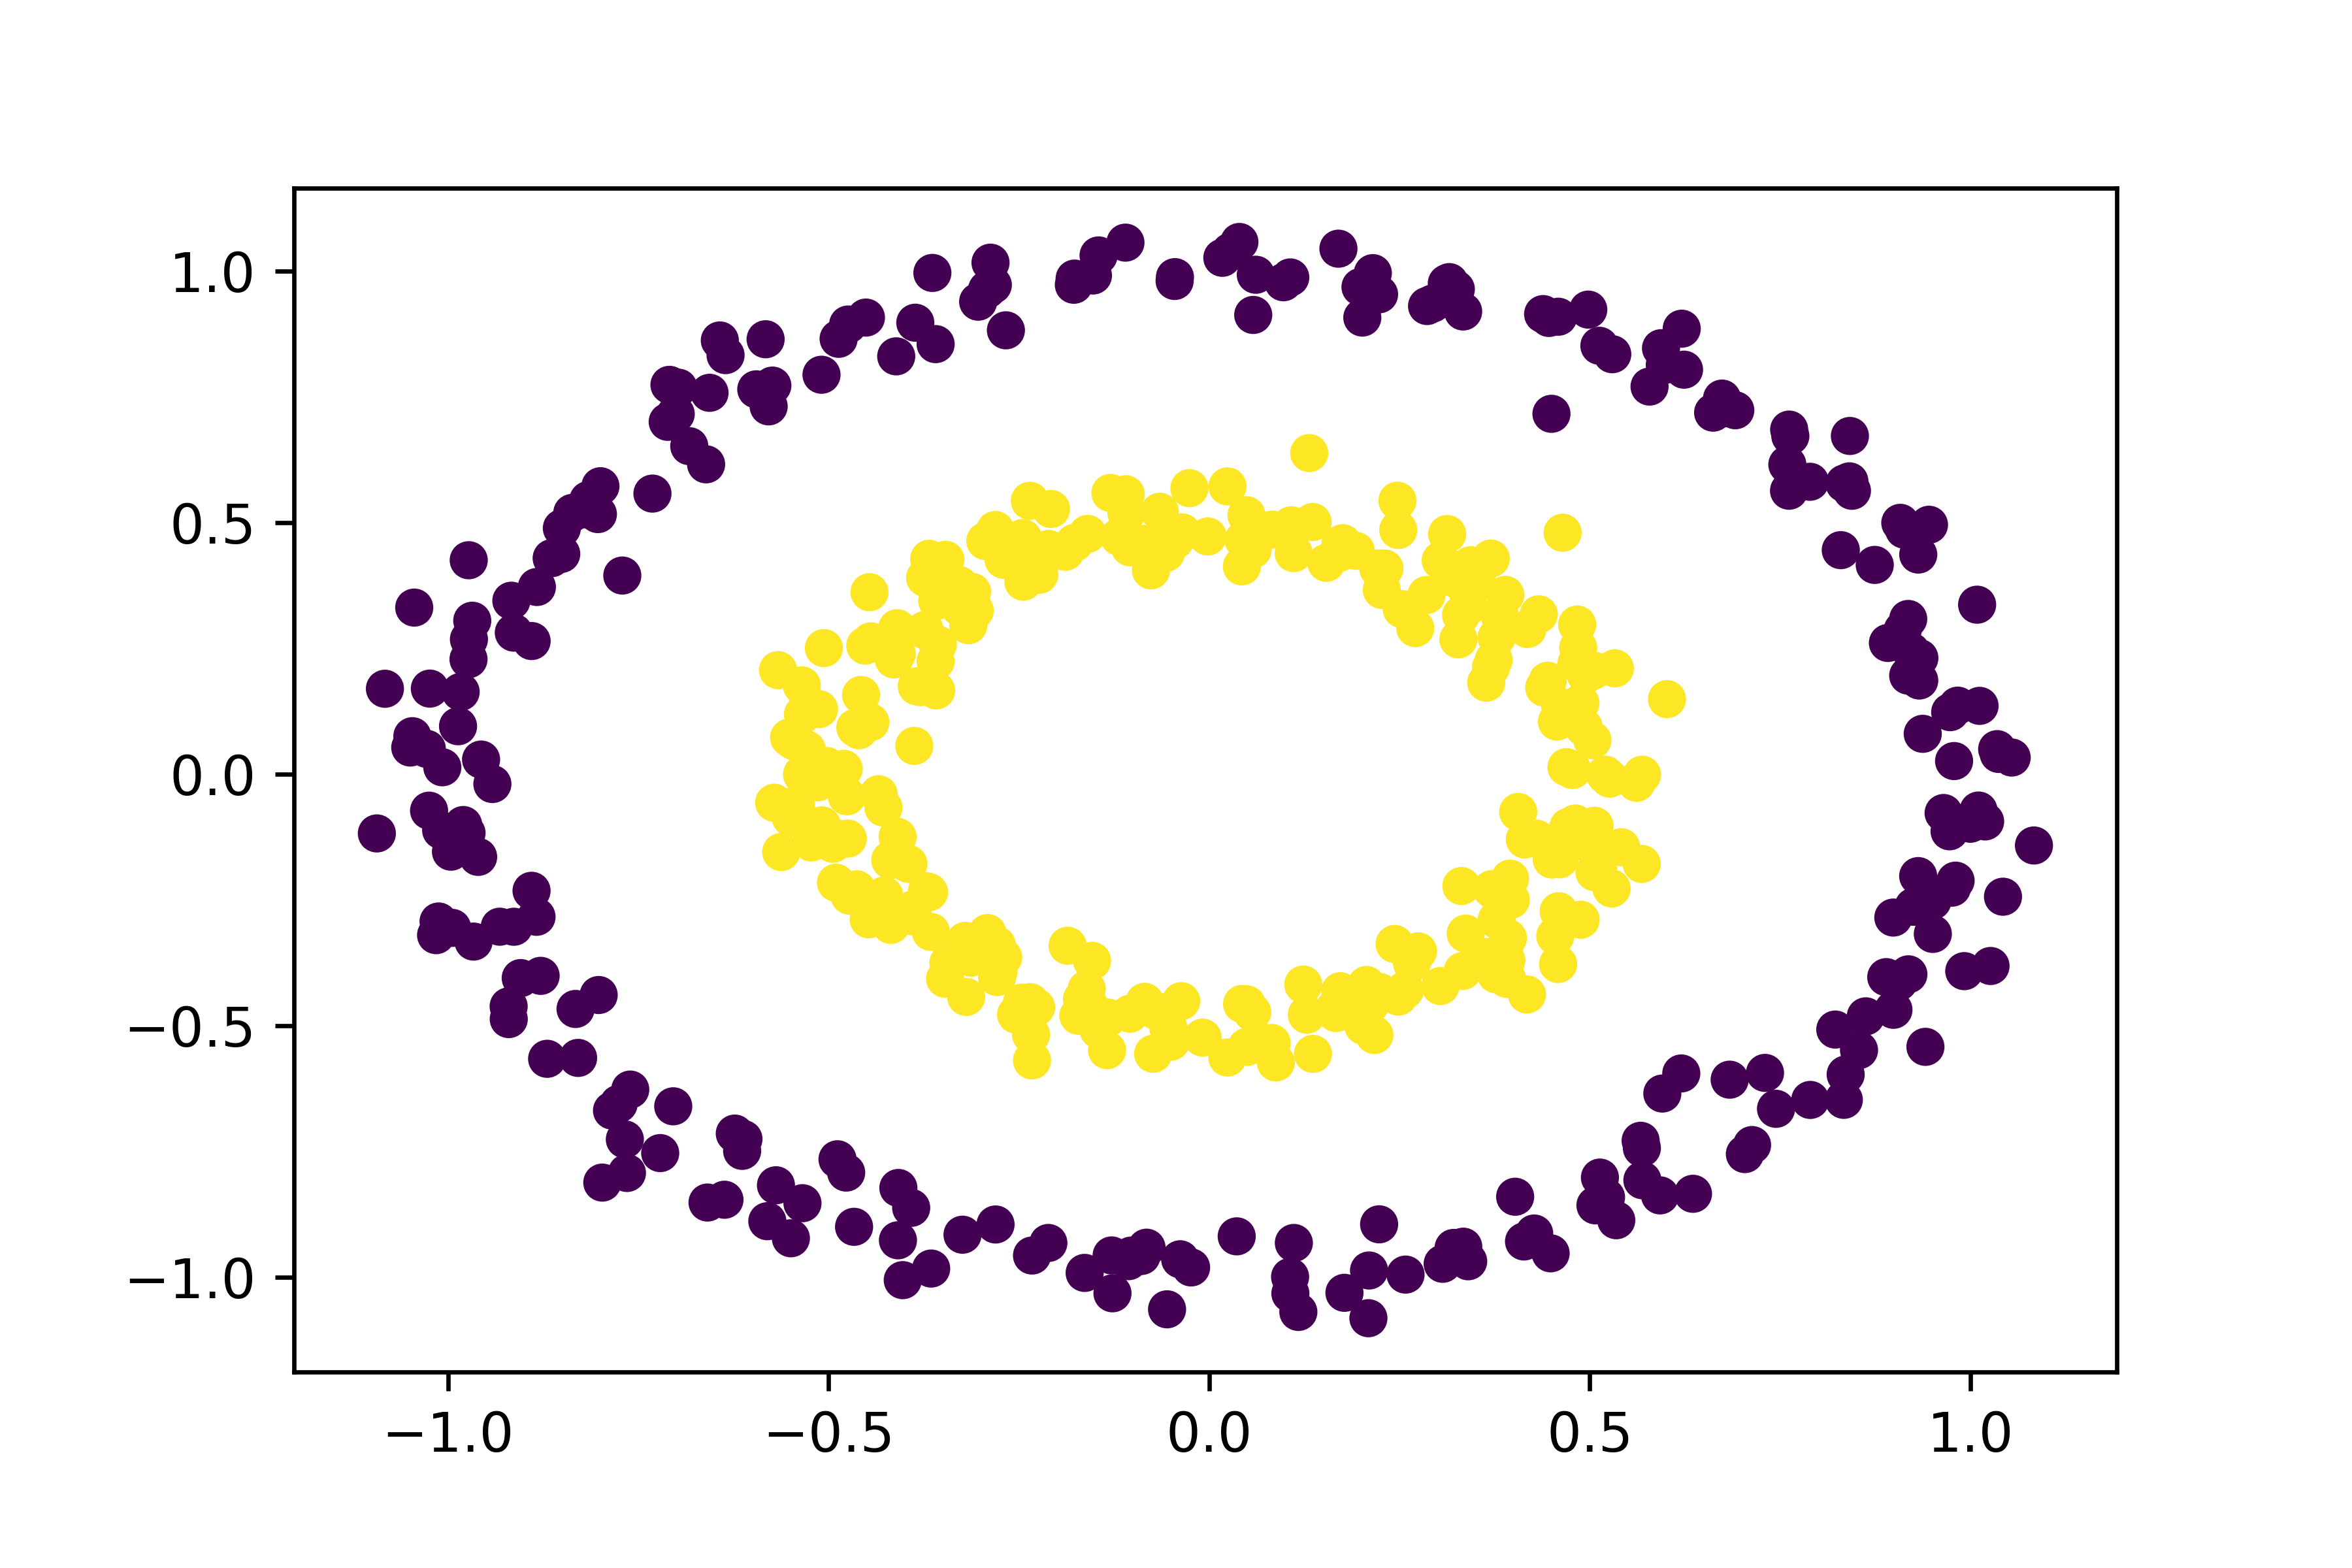
\includegraphics[width=0.55\linewidth]{d3.png}
    \caption{Original Dataset and expected cluster assignments}
\end{figure}%
\vspace*{-0.7cm}
\begin{figure}[H]
    \begin{subfigure}{0.33\linewidth}
        \centering
        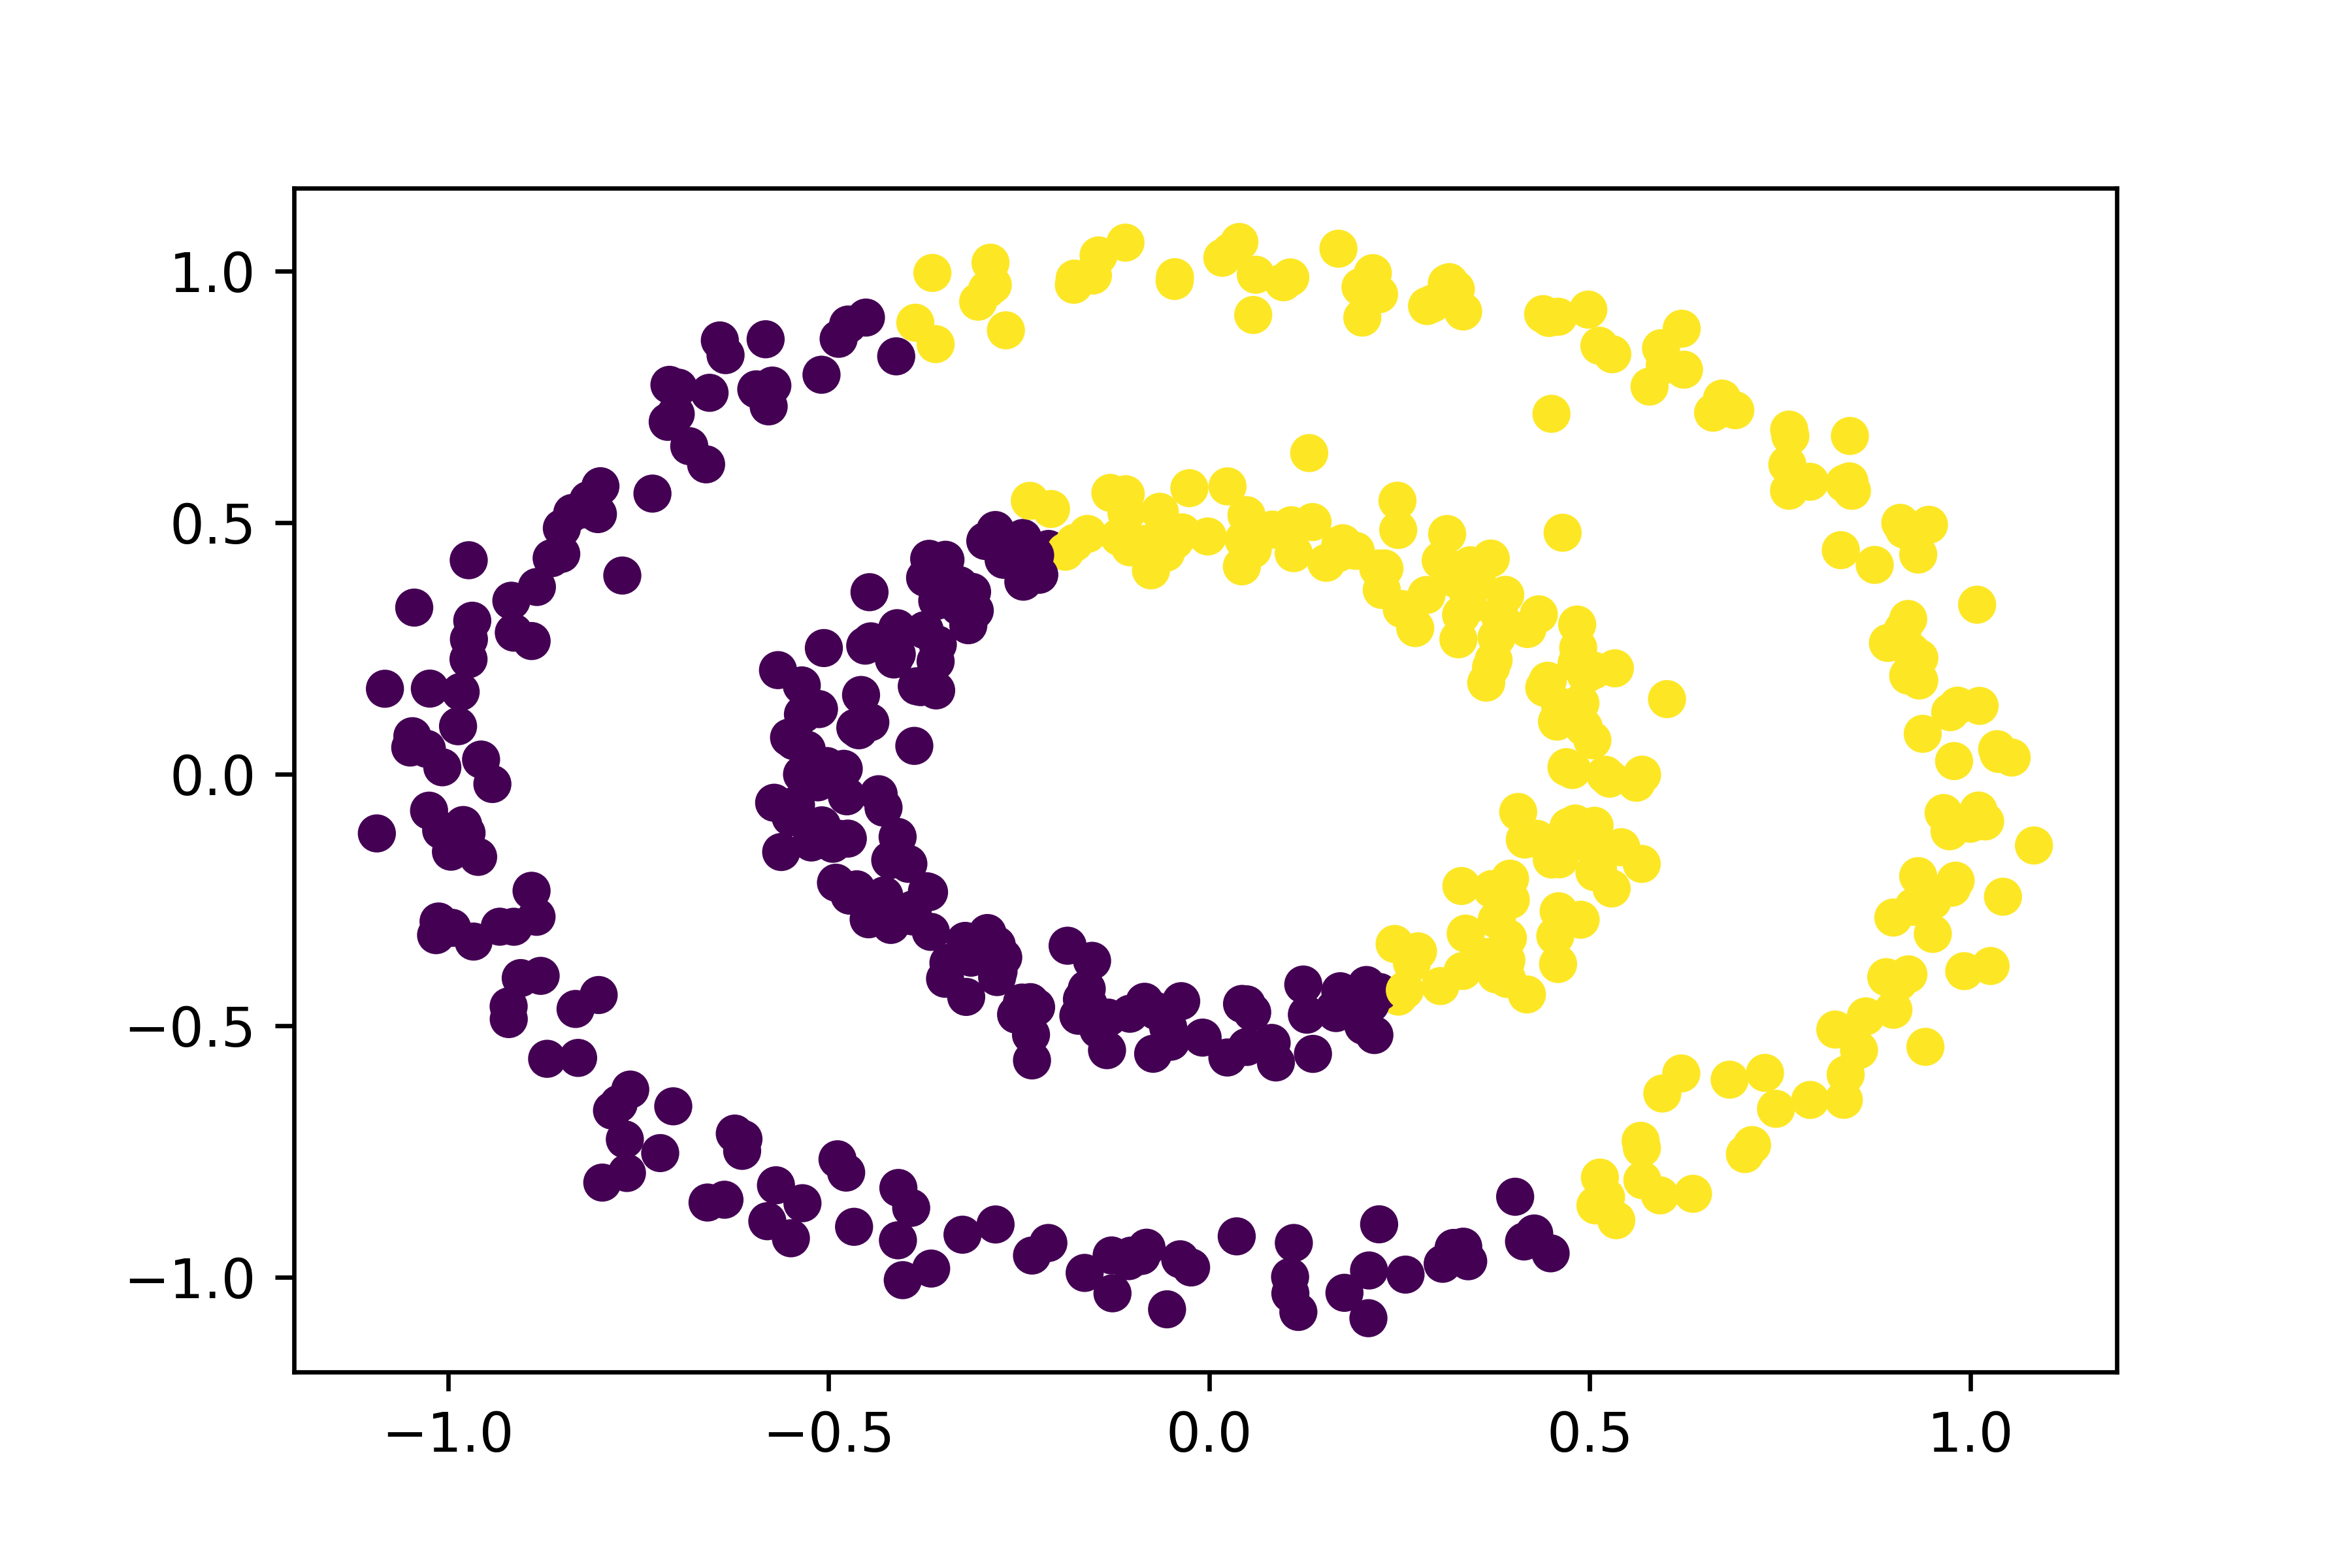
\includegraphics[width=1\linewidth]{d3_123.png}
        \caption{\textbf{SEED=123}}
    \end{subfigure}%
    \begin{subfigure}{0.33\linewidth}
        \centering
        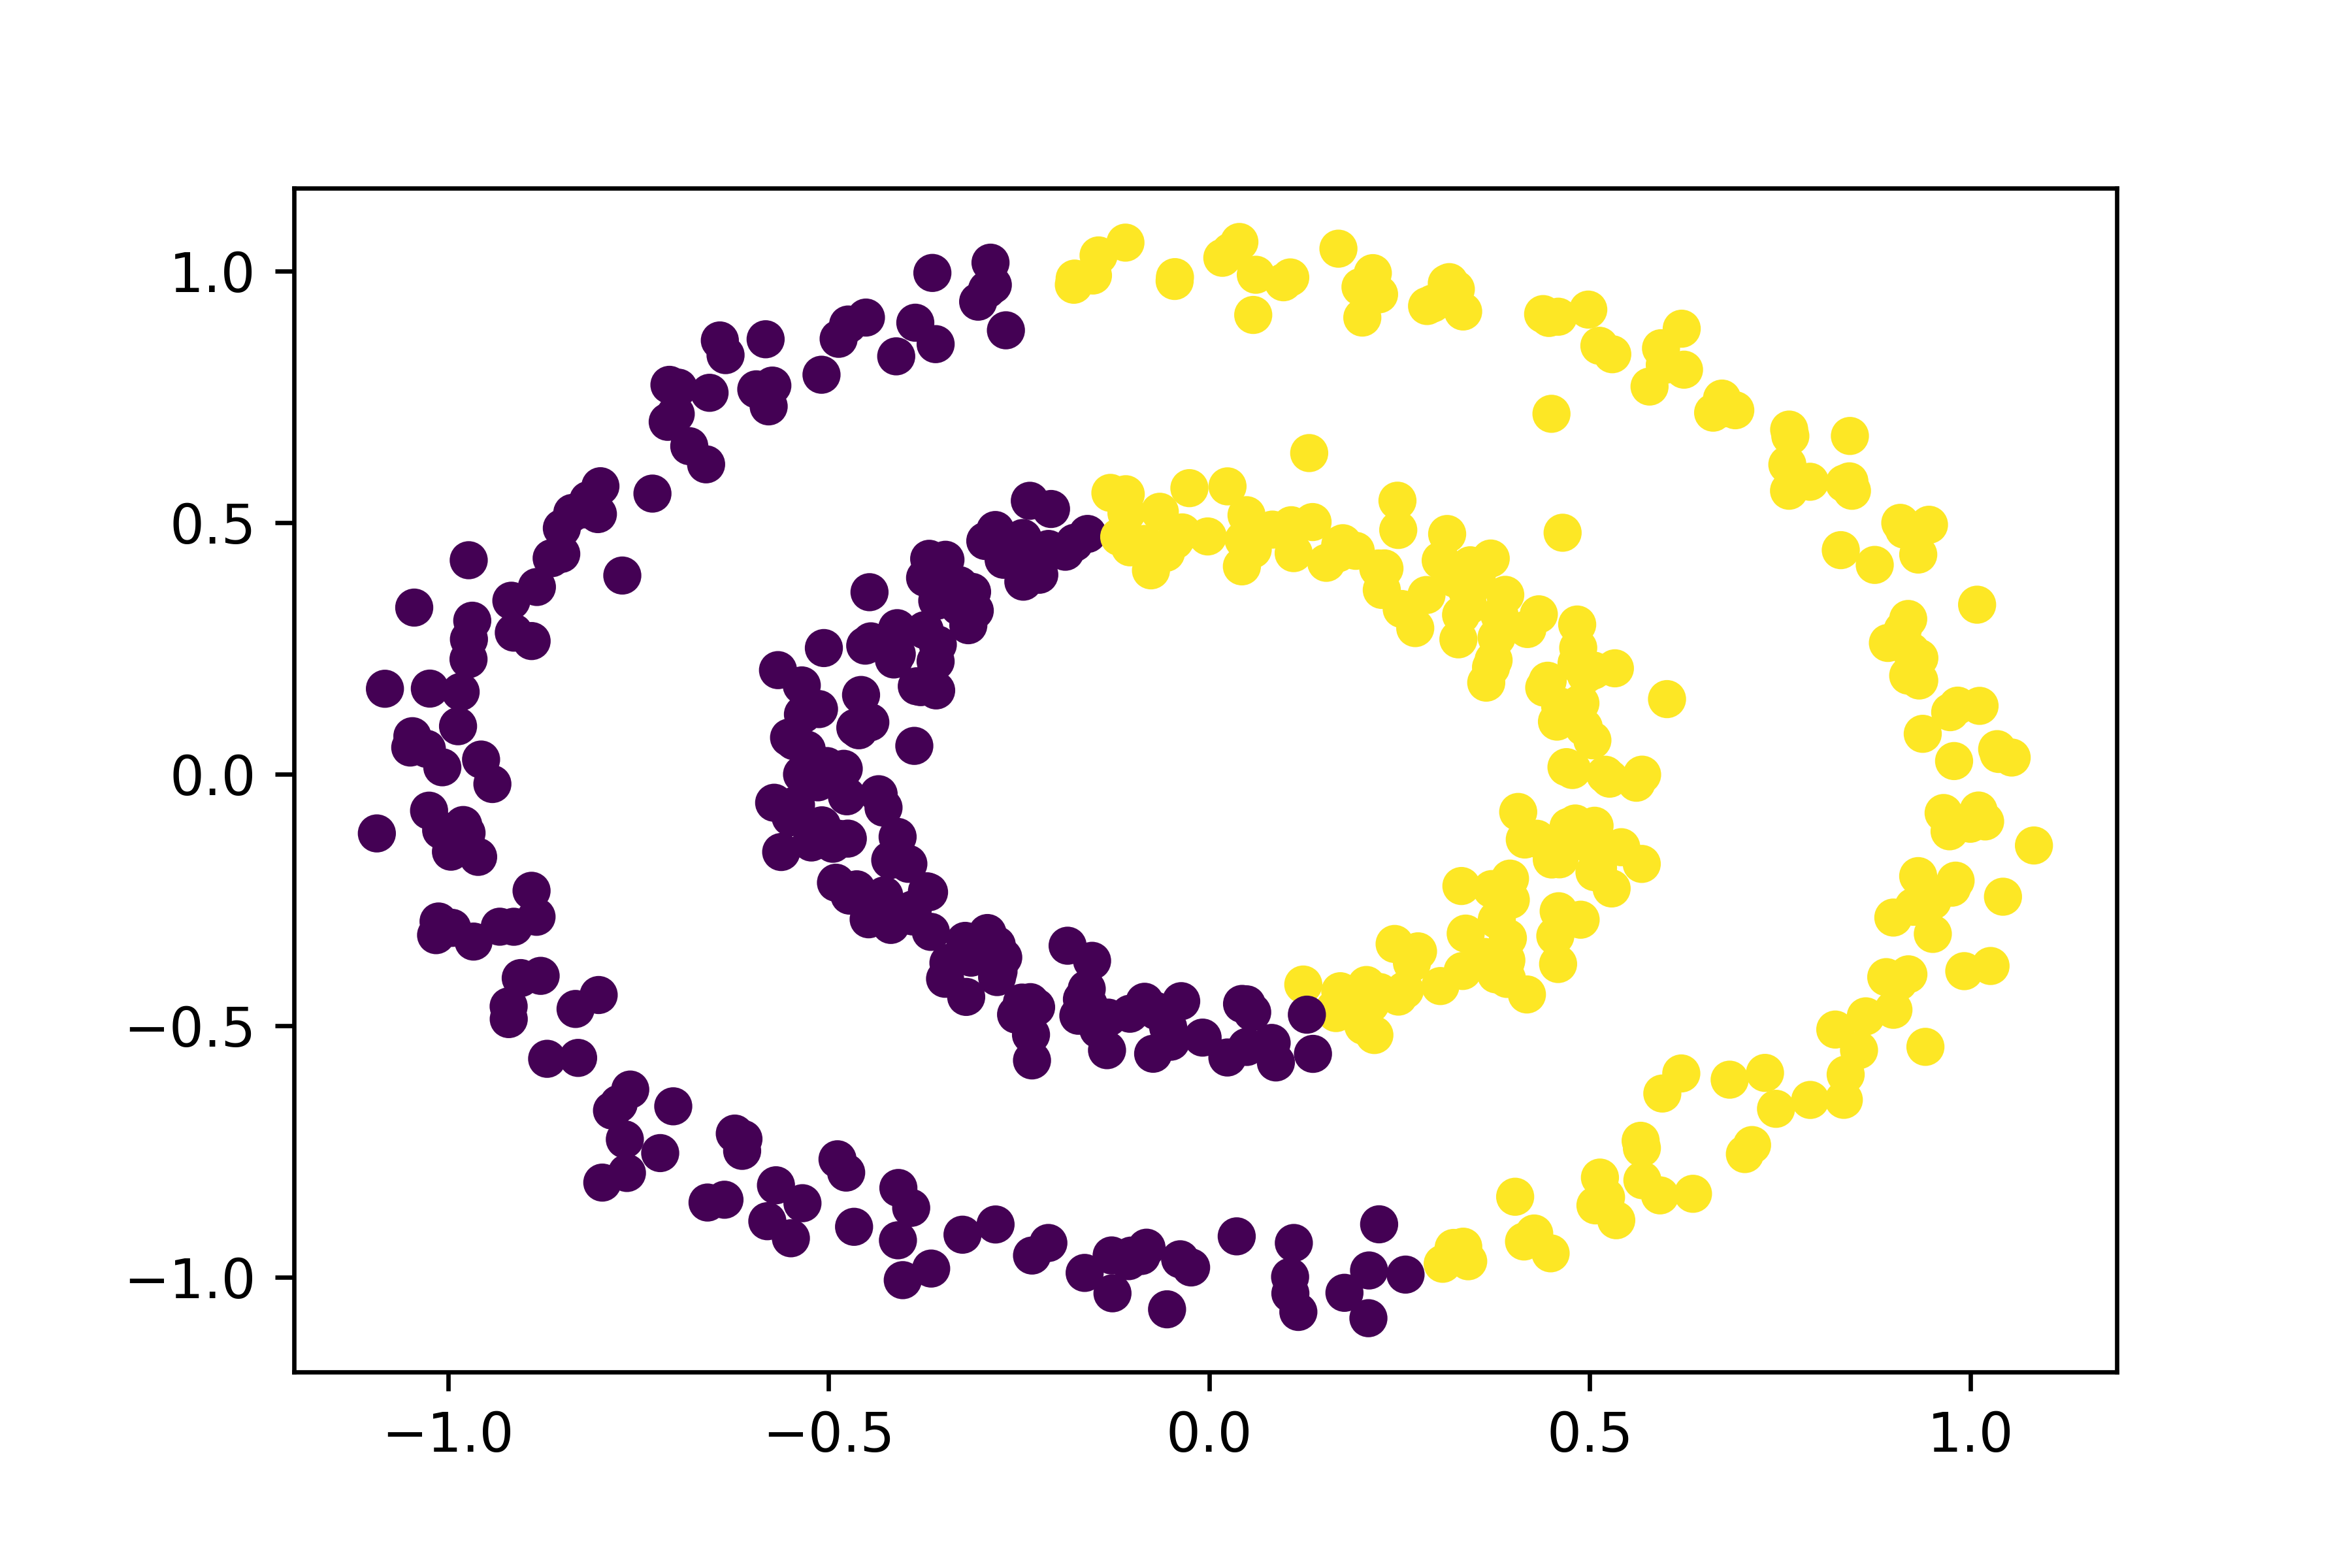
\includegraphics[width=1\linewidth]{d3_53641.png}
        \caption{\textbf{SEED=53641}}
    \end{subfigure}%
    \begin{subfigure}{0.33\linewidth}
        \centering
        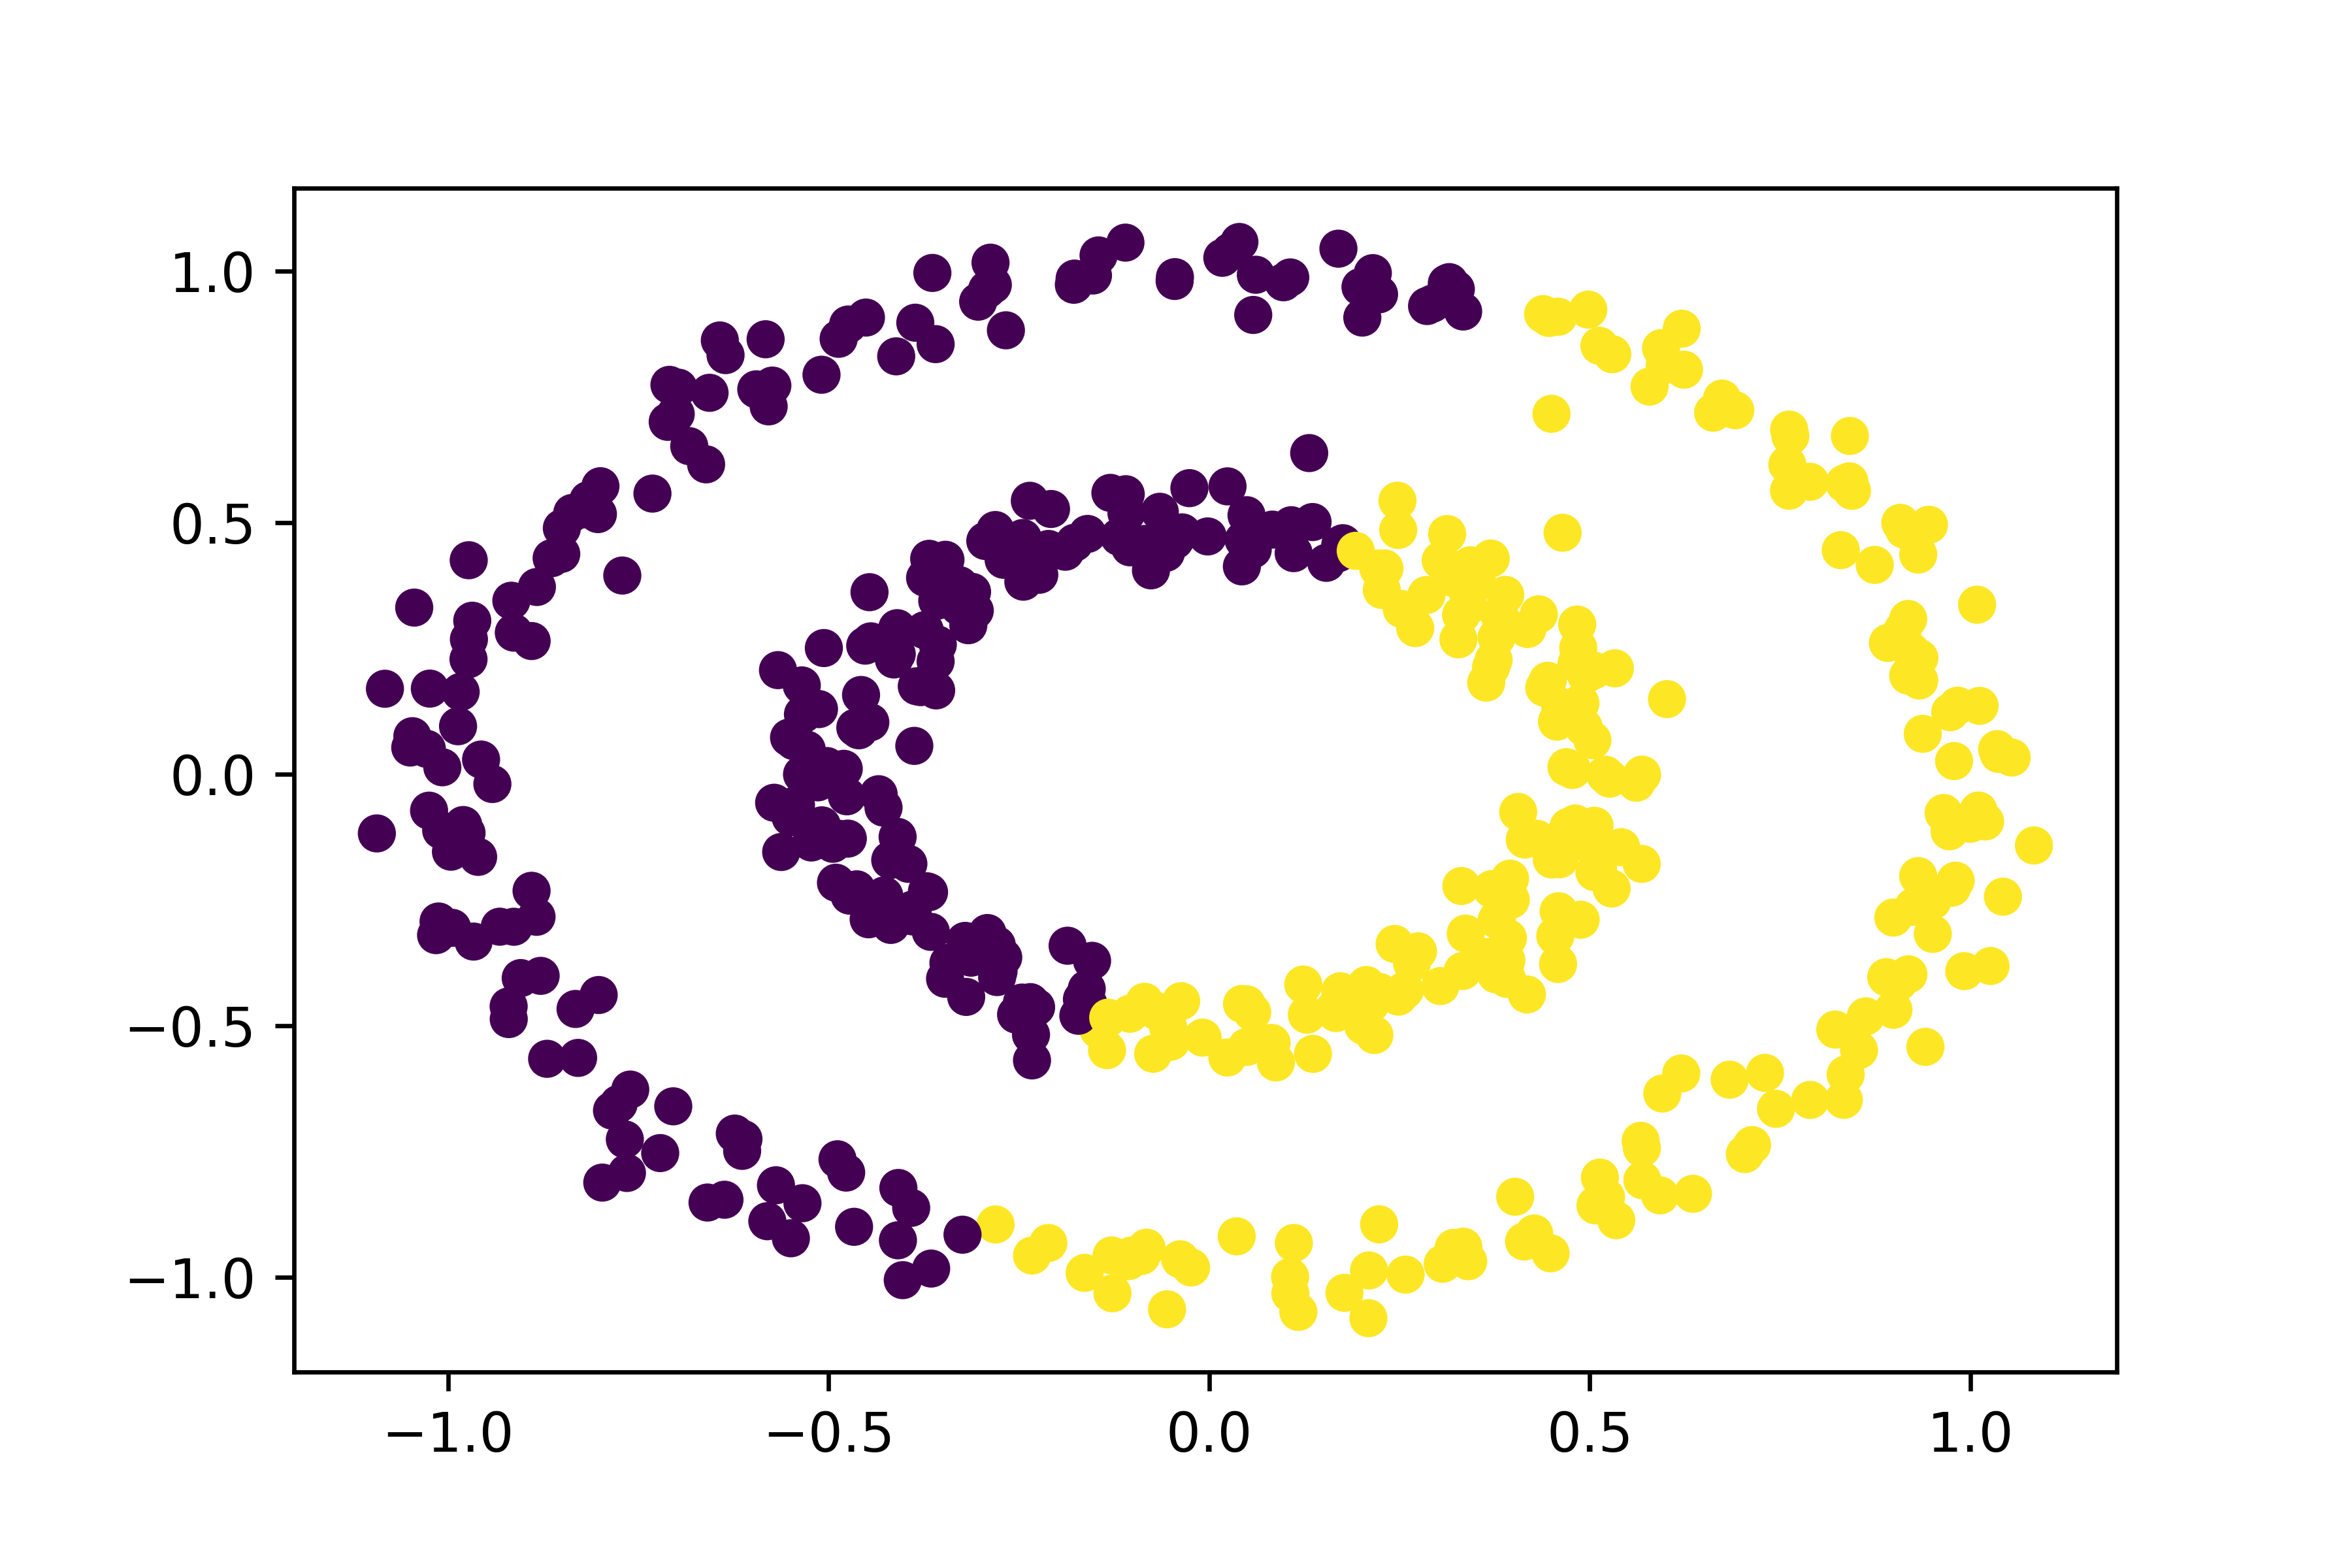
\includegraphics[width=1\linewidth]{d3_87234.png}
        \caption{\textbf{SEED=87234}}
    \end{subfigure}    
\end{figure}

\textbf{(iii)} Ideally we would want the cluster centre initialisations to be close to the true cluster centres. It should be at least in the same global minima bucket of the convex error function as the true cluster. But definitely we can't ensure this just by looking at the data. So we test out the following initialisation strategies:
\begin{itemize}
    \item[(a). ] \textbf{Randomly sample K data points as the K cluster centres:} 
        \begin{itemize}
            \item This is the strategy we adopt for this problem.
            
            \item It is easy to see the idea behind this. We would expect the true cluster centres to lie close to the mode of the cluster data points. So picking random data points as cluster centres seems plausible. 
            
            \item If random initialisation leads to two cluster centres getting initialised with data points lying in the same cluster, it is quite possible that this initialisation strategy will perform poorly. So we also explore another algorithm.  
        \end{itemize}
    
    \item[(b). ] \textbf{kmeans++ :} \href{https://theory.stanford.edu/~sergei/papers/kMeansPP-soda.pdf}{[link to publication]} \href{https://medium.com/analytics-vidhya/comparison-of-initialization-strategies-for-k-means-d5ddd8b0350e#:~:text=using%20this%20method.-,kmeans%2B%2B,-This%20is%20a}{[Link to a reference used to understand this topic]}. The basic idea here is to choose the initial points far apart from each other (but with some differences with the Farthest Point Method). As they outline:
        \begin{itemize}
            \item We start this initialisation procedure like the previously outlined one (that is by choose random points from the data). 
            
            \item We choose the following points such that its likely to lie at a large distance from its previously assigned set of points. They perform the sampling of the point from a probability distribution that is proportional to the squared distance of a point from the first centre.
            
            \item The remaining points are generated by a probability distribution that is proportional to the squared distance of each point from its closest centre. So, a point having a large distance from its closest centre is more likely to be sampled.
        \end{itemize}
    But this method takes up additional computational capacity to build the initial cluster centres. We choose to go for \textbf{(a)} as described above for this assignment.
\end{itemize}


\section{\texttt{Kernel design and Kernelized clustering}}

\subsection{\texttt{CS 337: Proving kernel validity}}

Prove that the function $K_{\sigma} : \mathbb{R}^{n} \times \mathbb{R}^{n} \longrightarrow \mathbb{R}$ defined as $K_{\sigma} (\mathbf{x}, \mathbf{y}) = \exp\left( \frac{-\lVert x-y \rVert^{2}}{2\sigma^{2}} \right)$ is a valid Kernel. 

\textit{Solution. } 

We will use \textbf{sum, product and positive scaling closure} properties of Kernels to prove this. 

\textbf{Observation: } \textit{If $K(x,y)$ is a valid kernel then $\exp\left(K(x,y)\right)$ is also a valid kernel.}

\textbf{Proof: } We can use Taylor's expansion around 0.%
\begin{gather*}
   \exp\left( K(x,y) \right) = 1 + K + \frac{K^2}{2} + \frac{K^3}{6} + \cdots \\
   = \sum_{i=0}^{\infty} \frac{K(x,y)^{i}}{i!}
\end{gather*}

\textbf{By product and positive scaling closure} properties every term of the summation is a valid kernel, i.e. $K(x,y)^{i}$ is a valid kernel because $K(x,y)$ is a valid kernel. Also, $\frac{1}{i!} > 0$, so $\frac{K(x,y)^{i}}{i!}$ is a valid kernel.

Therefore $\exp\left(K(x,y)\right)$ is a valid kernel.

\textbf{Now,} since $\exp\left(K(x,y)\right)$ is a kernel, by \textbf{Mercer's Theorem}, $\exists$ a feature map $\phi(\mathbf{x}) : \mathbb{R}^{n} \rightarrow \mathrm{H}$, s.t.%
\begin{equation*}
    \exp\left(K(x,y)\right) = \phi(x)^{T}\phi(y)
\end{equation*}%
where, $\mathrm{H}$ is a Hilbert space.


\textbf{Now,} the given kernel: %
\begin{gather*}
    \exp\left( \frac{-\lVert x-y \rVert^{2}}{2\sigma^{2}} \right) = \exp\left( \frac{-\lVert x \rVert^{2} -\lVert x \rVert^{2} + 2x^{T}y}{2\sigma^{2}} \right) \\
    = \exp\left( \frac{-\lVert x \rVert^{2}}{2\sigma^{2}} \right) \times \exp\left( \frac{-\lVert y \rVert^{2}}{2\sigma^{2}} \right) \times \exp\left( \frac{x^{T}y}{\sigma^{2}} \right)
\end{gather*}

We know that $x^{T}y$ is a valid kernel with an identity feature map. Given $\sigma^{2} > 0$, we know $\frac{x^{T}y}{\sigma^2}$ is also a valid kernel. This means, $\exists \, \phi$ s.t. %
\begin{equation*}
    \exp\left( \frac{x^{T}y}{\sigma^2} \right) = \phi(x)^{T}\phi(y)
\end{equation*}

Therefore, rewriting the kernel we get,%
\begin{gather*}
    \exp\left( \frac{-\lVert x-y \rVert^{2}}{2\sigma^{2}} \right) = \exp\left( \frac{-\lVert x \rVert^{2}}{2\sigma^{2}} \right) \times \phi(x)^{T}\phi(y) \times \exp\left( \frac{-\lVert y \rVert^{2}}{2\sigma^{2}} \right) \\
    = \left( \phi(x)\exp\left( \frac{-\lVert x \rVert^{2}}{2\sigma^{2}} \right) \right)^{T} \left( \phi(y)\exp\left( \frac{-\lVert y \rVert^{2}}{2\sigma^{2}} \right) \right)
\end{gather*}

Therefore, we can construct the projection space of the given kernel $\phi^{'}(x) = \phi(x)\exp\left( \frac{-\lVert x \rVert^{2}}{2\sigma^{2}} \right)$. Since a valid feature map exists, the given kernel is a valid kernel!


\subsection{\texttt{CS 337: Simple Kernel Design}}

\textbf{1. } \textit{Is there a condition on $r_1$ , $r_2$ such that the vanilla KMeans (vanilla means we need to run the algorithm as is on the given data without transformations of any kind) algorithm gives us the correct clusters?}

\textit{Solution: } 

No, there does not exist a pair of $r_1$, $r_2$ such that vanilla KMeans algorithm gives us the correct clusters. This is because K-Means cannot cluster non-convex datasets.

\textbf{Proof: } We propose a proof by contradiction for the given concentric dataset case. Let 2 distinct cluster centers $c_1$(for $r_1$) and $c_2$ (for $r_2$) be such that K-means can perfectly cluster the dataset, after we are done with the \textit{fit()} function.
 
Wlog assume $r_2 < r_1$. Assume $c_i < r_i$ means cluster center $c_i$ lies inside circle with radius $r_i$. We consider the following \textbf{cases}:%
\begin{enumerate}
    \item $c_1 < r_2$ and $c_2 < r_2$: If we take the line joining $c_1$ and $c_2$, it will intersect the inner circle at points $p_1$ and $p_2$. As, $p_1$ and $p_2$ belong to the cluster corresponding to $c_2$, their distances from $c_2$ should be less than their corresponding distances from $c_1$. Since straight line gives us the shortest distance, it is obvious that the above claim will lead to a contradiction.
    
    \item $r_2 < c_1 < r_1$ and $c_2 > r_1$: The line joining $c_1$ and $c_2$ intersect the outer circle. Let $p_1$ lies between $c_1$ and $c_2$ and $p_2$ lies on the opposite. Both of these points should lie closer to $c_1$, but again that leads to a contradiction. 
    
    \item $r_2 < c_2 < r_1$ and $c_1 > r_1$: Follows the same idea.
    
    \item $c_1 > r_1$ and $c_2 > r_1$: The point on the outer circle that lies on the line joining the origin and $c_2$. This point is closer to $c_2$ than $c_1$, giving a contradiction.
\end{enumerate}

Therefore, using exhaustive cases, we have shown that for any $r_1$, $r_2$ and corresponding $c_1$, $c_2$ vanilla K-Means won't be able to correctly cluster the given dataset of concentric circles.




\textbf{2. } \textit{For the configurations of $r_1$ , $r_2$ that are not clusterable, can you suggest a kernel that will help KMeans identify the correct clusters? Specify both the transformation $\phi(x)$ and the kernel function $k(x, x')$. Further show that the kernel function you propose is a valid kernel.}

\textit{Solution: } 

The basic intuition for formulating a good kernel for clustering concentric circles is to utilise the similar radius of the data points lying in a particular cluster. To use the radius of the clusters for clustering, we can use $\lVert x \rVert_{2}^{2}$ as the cluster metric. We will \textbf{first propose the kernel} and derive its \textbf{transformation space} $\boldsymbol{\phi(x)}$.


We propose the following {\color{red}\textbf{kernel}}:%
\begin{equation}
    k(x, x') = \exp\left( \gamma \left( \lVert x \rVert_{2} + \lVert y \rVert_{2} \right) \right)
\end{equation}
 
Let's derive the \textbf{transformation space} for this proposed kernel:%
\begin{gather*}
    k(x, x') = \exp\left( \gamma \left( \lVert x \rVert + \lVert y \rVert \right) \right) \\
    = \exp\left( \gamma \lVert x \rVert \right) \exp\left( \gamma \lVert y \rVert \right) 
\end{gather*} 
Therefore, the {\color{red}\textbf{transformation space}} is $\boldsymbol{\phi(x) = \exp\left( \gamma \lVert x \rVert_{2} \right)}$, since we assume $\lVert x \rVert$ is a scalar under the current problem settings.%
\begin{equation*}
    k(x, x') = \langle \phi(x), \phi(y) \rangle = \phi(x)^{T}\phi(y) = \exp\left( \gamma \lVert x \rVert \right) \exp\left( \gamma \lVert y \rVert \right)
\end{equation*}
since the transformation is from $\mathbb{R}^{2} \longrightarrow \mathbb{R}$


\underline{\textbf{Proof - Proposed kernel is a Mercer Kernel (hence valid): }}

By theorem, a kernel $K(x, y)$ is a Mercer kernel if $\int_{x} \int_{y} K(x, y) g(x) g(y) dx dy \geq 0$ for all square integrable functions $g(x)$.

Therefore,%
\begin{gather*}
    \int_{x} \int_{y} K(x, y) g(x) g(y) dx dy = \int_{x} \int_{y} \exp\left( \gamma \left( \lVert x \rVert_{2} + \lVert y \rVert_{2} \right) \right) g(x) g(y) dx dy \\
    = \int_{x} \int_{y} \exp\left( \gamma \lVert x \rVert \right) \exp\left( \gamma \lVert y \rVert \right)  g(x) g(y) dx dy \\
\end{gather*}%
Using Fubini's Theorem we can write the iterated integral as a product of integrals:%
\begin{gather*}
    \int_{x} \int_{y} \exp\left( \gamma \lVert x \rVert \right) \exp\left( \gamma \lVert y \rVert \right)  g(x) g(y) dx dy = \int_{x} \exp\left( \gamma \lVert x \rVert \right) g(x) dx \int_{y} \exp\left( \gamma \lVert y \rVert \right) g(y) dy \\
    = \left( \int_{x} \exp\left( \gamma \lVert x \rVert \right) g(x) dx \right)^{2} \geq 0
\end{gather*}
Therefore our proposed kernel is a Mercer Kernel and valid.

\underline{\textbf{Results with this kernel: }}

\begin{figure}[H]
    \centering
    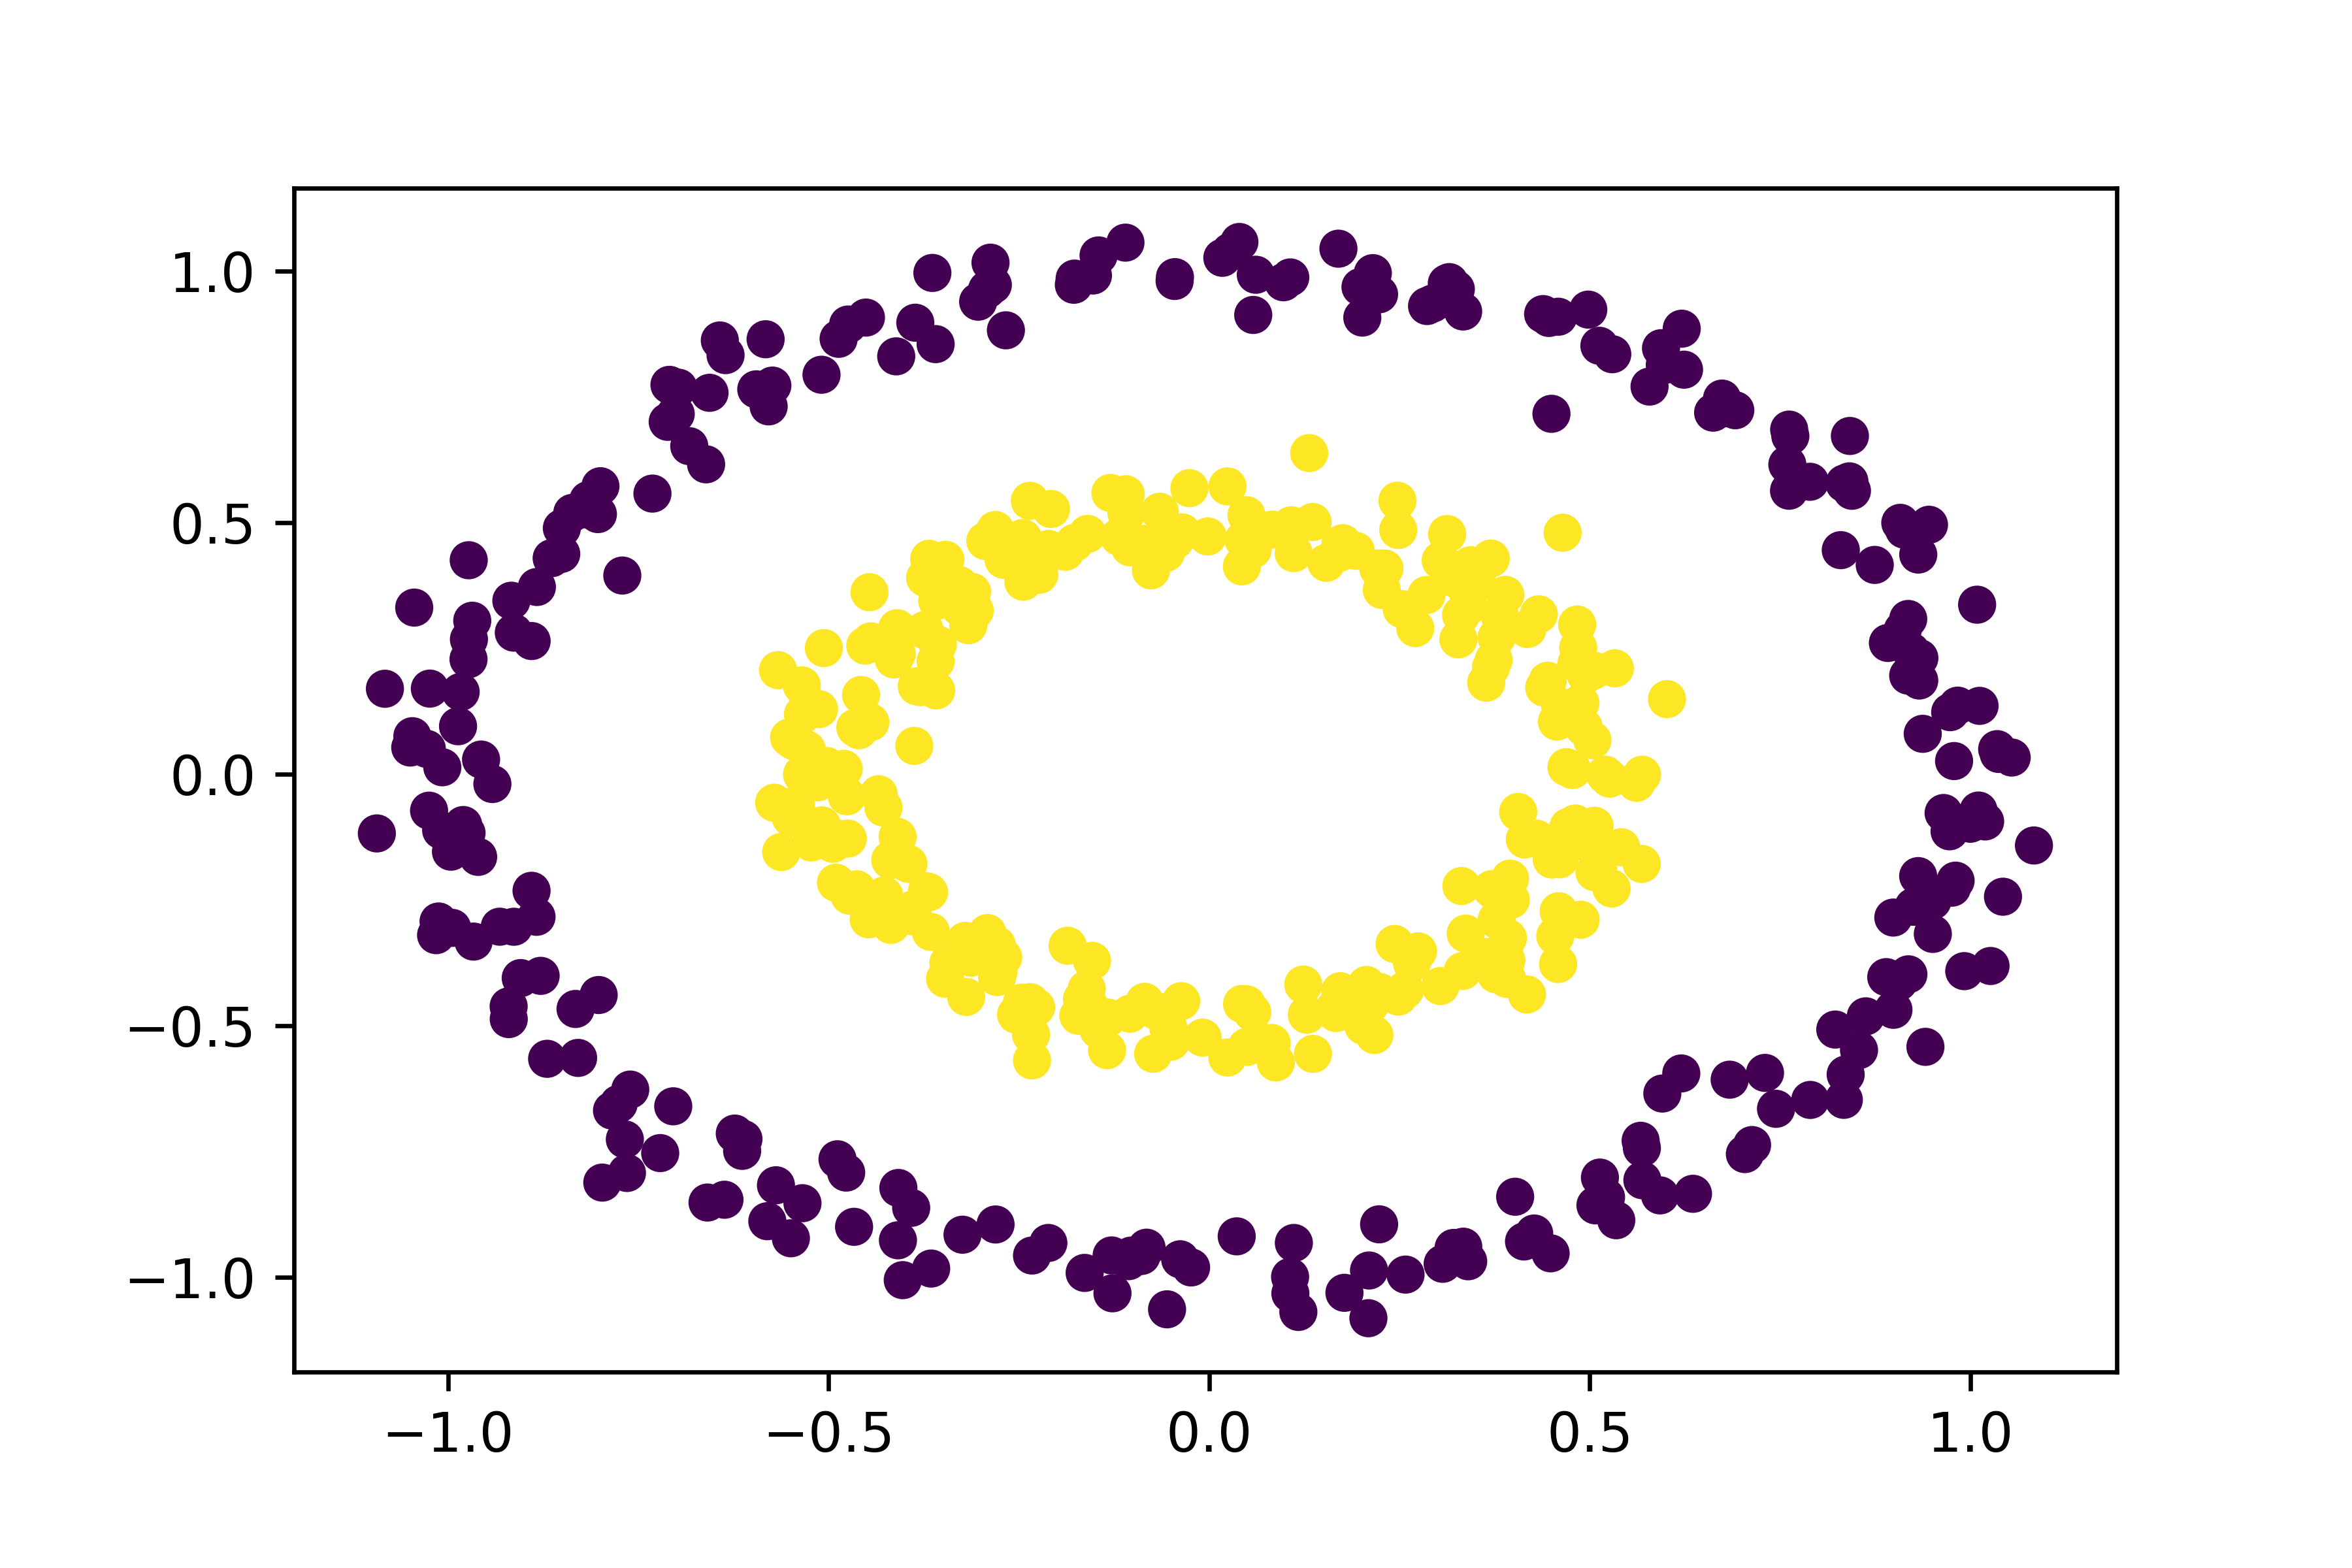
\includegraphics[width=0.55\linewidth]{kkm.png}
    \caption{Original Dataset and expected cluster assignments}
\end{figure}%
\vspace*{-0.7cm}
\begin{figure}[H]
    \begin{subfigure}{0.33\linewidth}
        \centering
        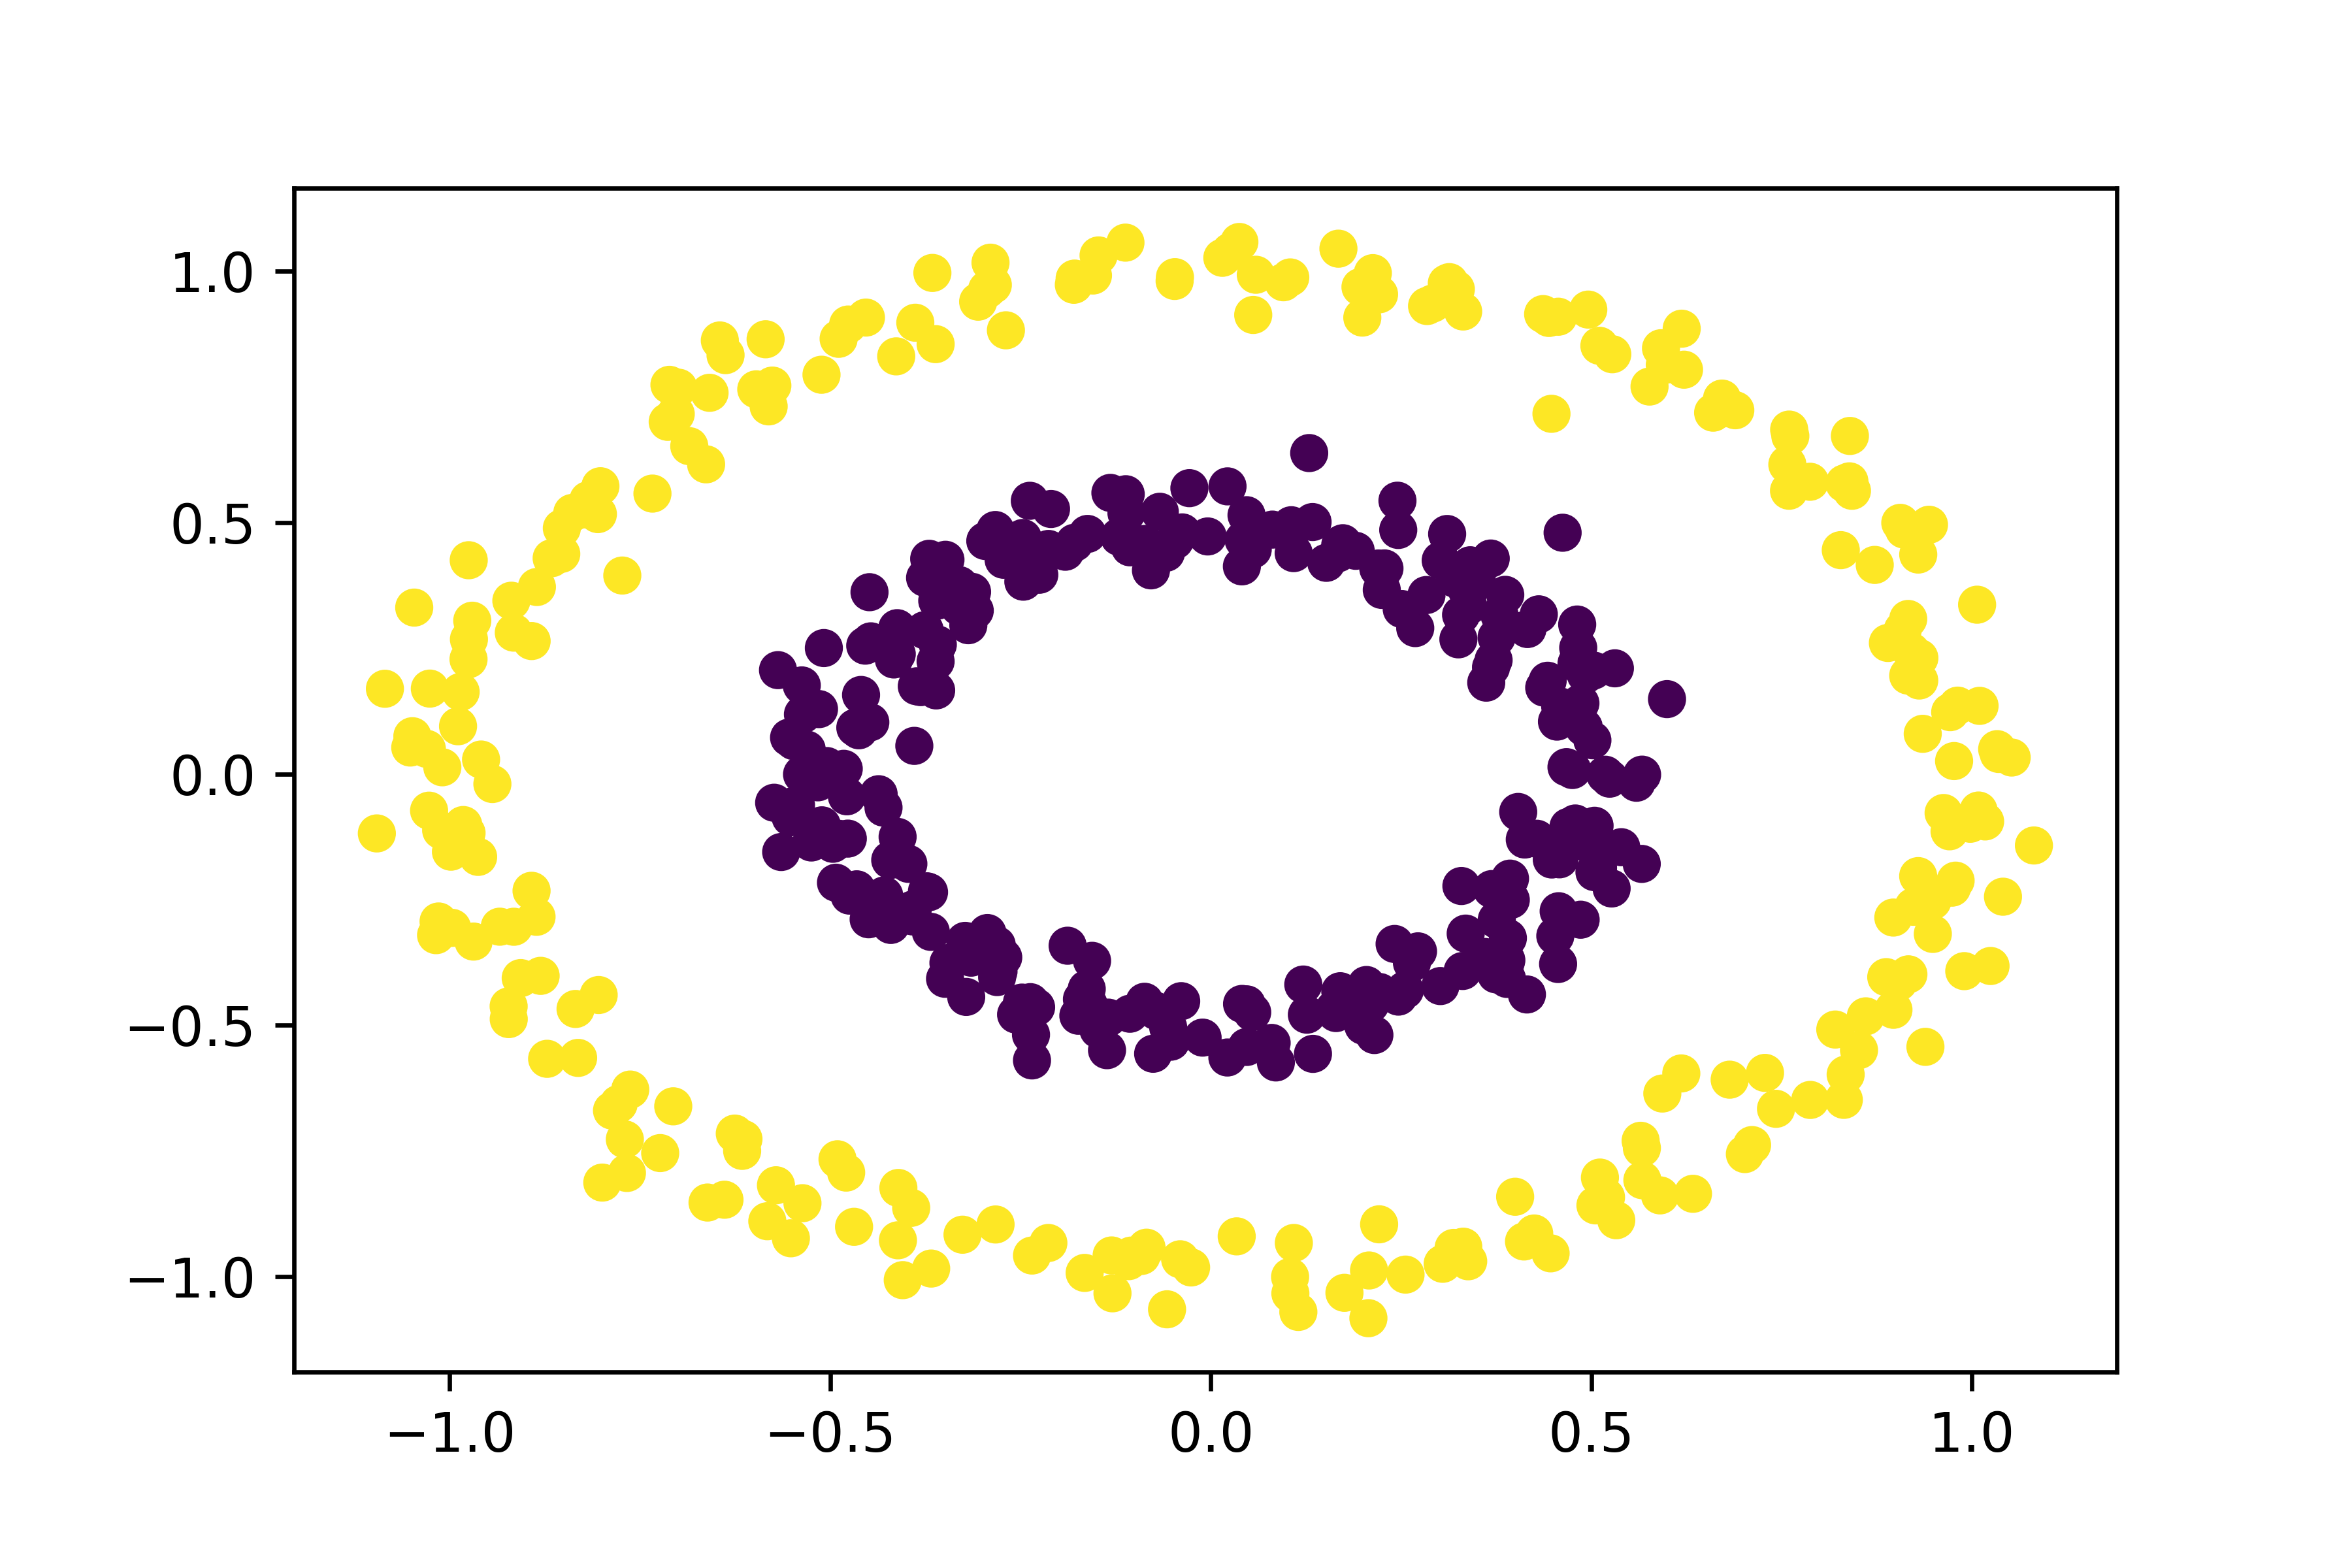
\includegraphics[width=1\linewidth]{kkm_123.png}
        \caption{\textbf{SEED=123}}
    \end{subfigure}%
    \begin{subfigure}{0.33\linewidth}
        \centering
        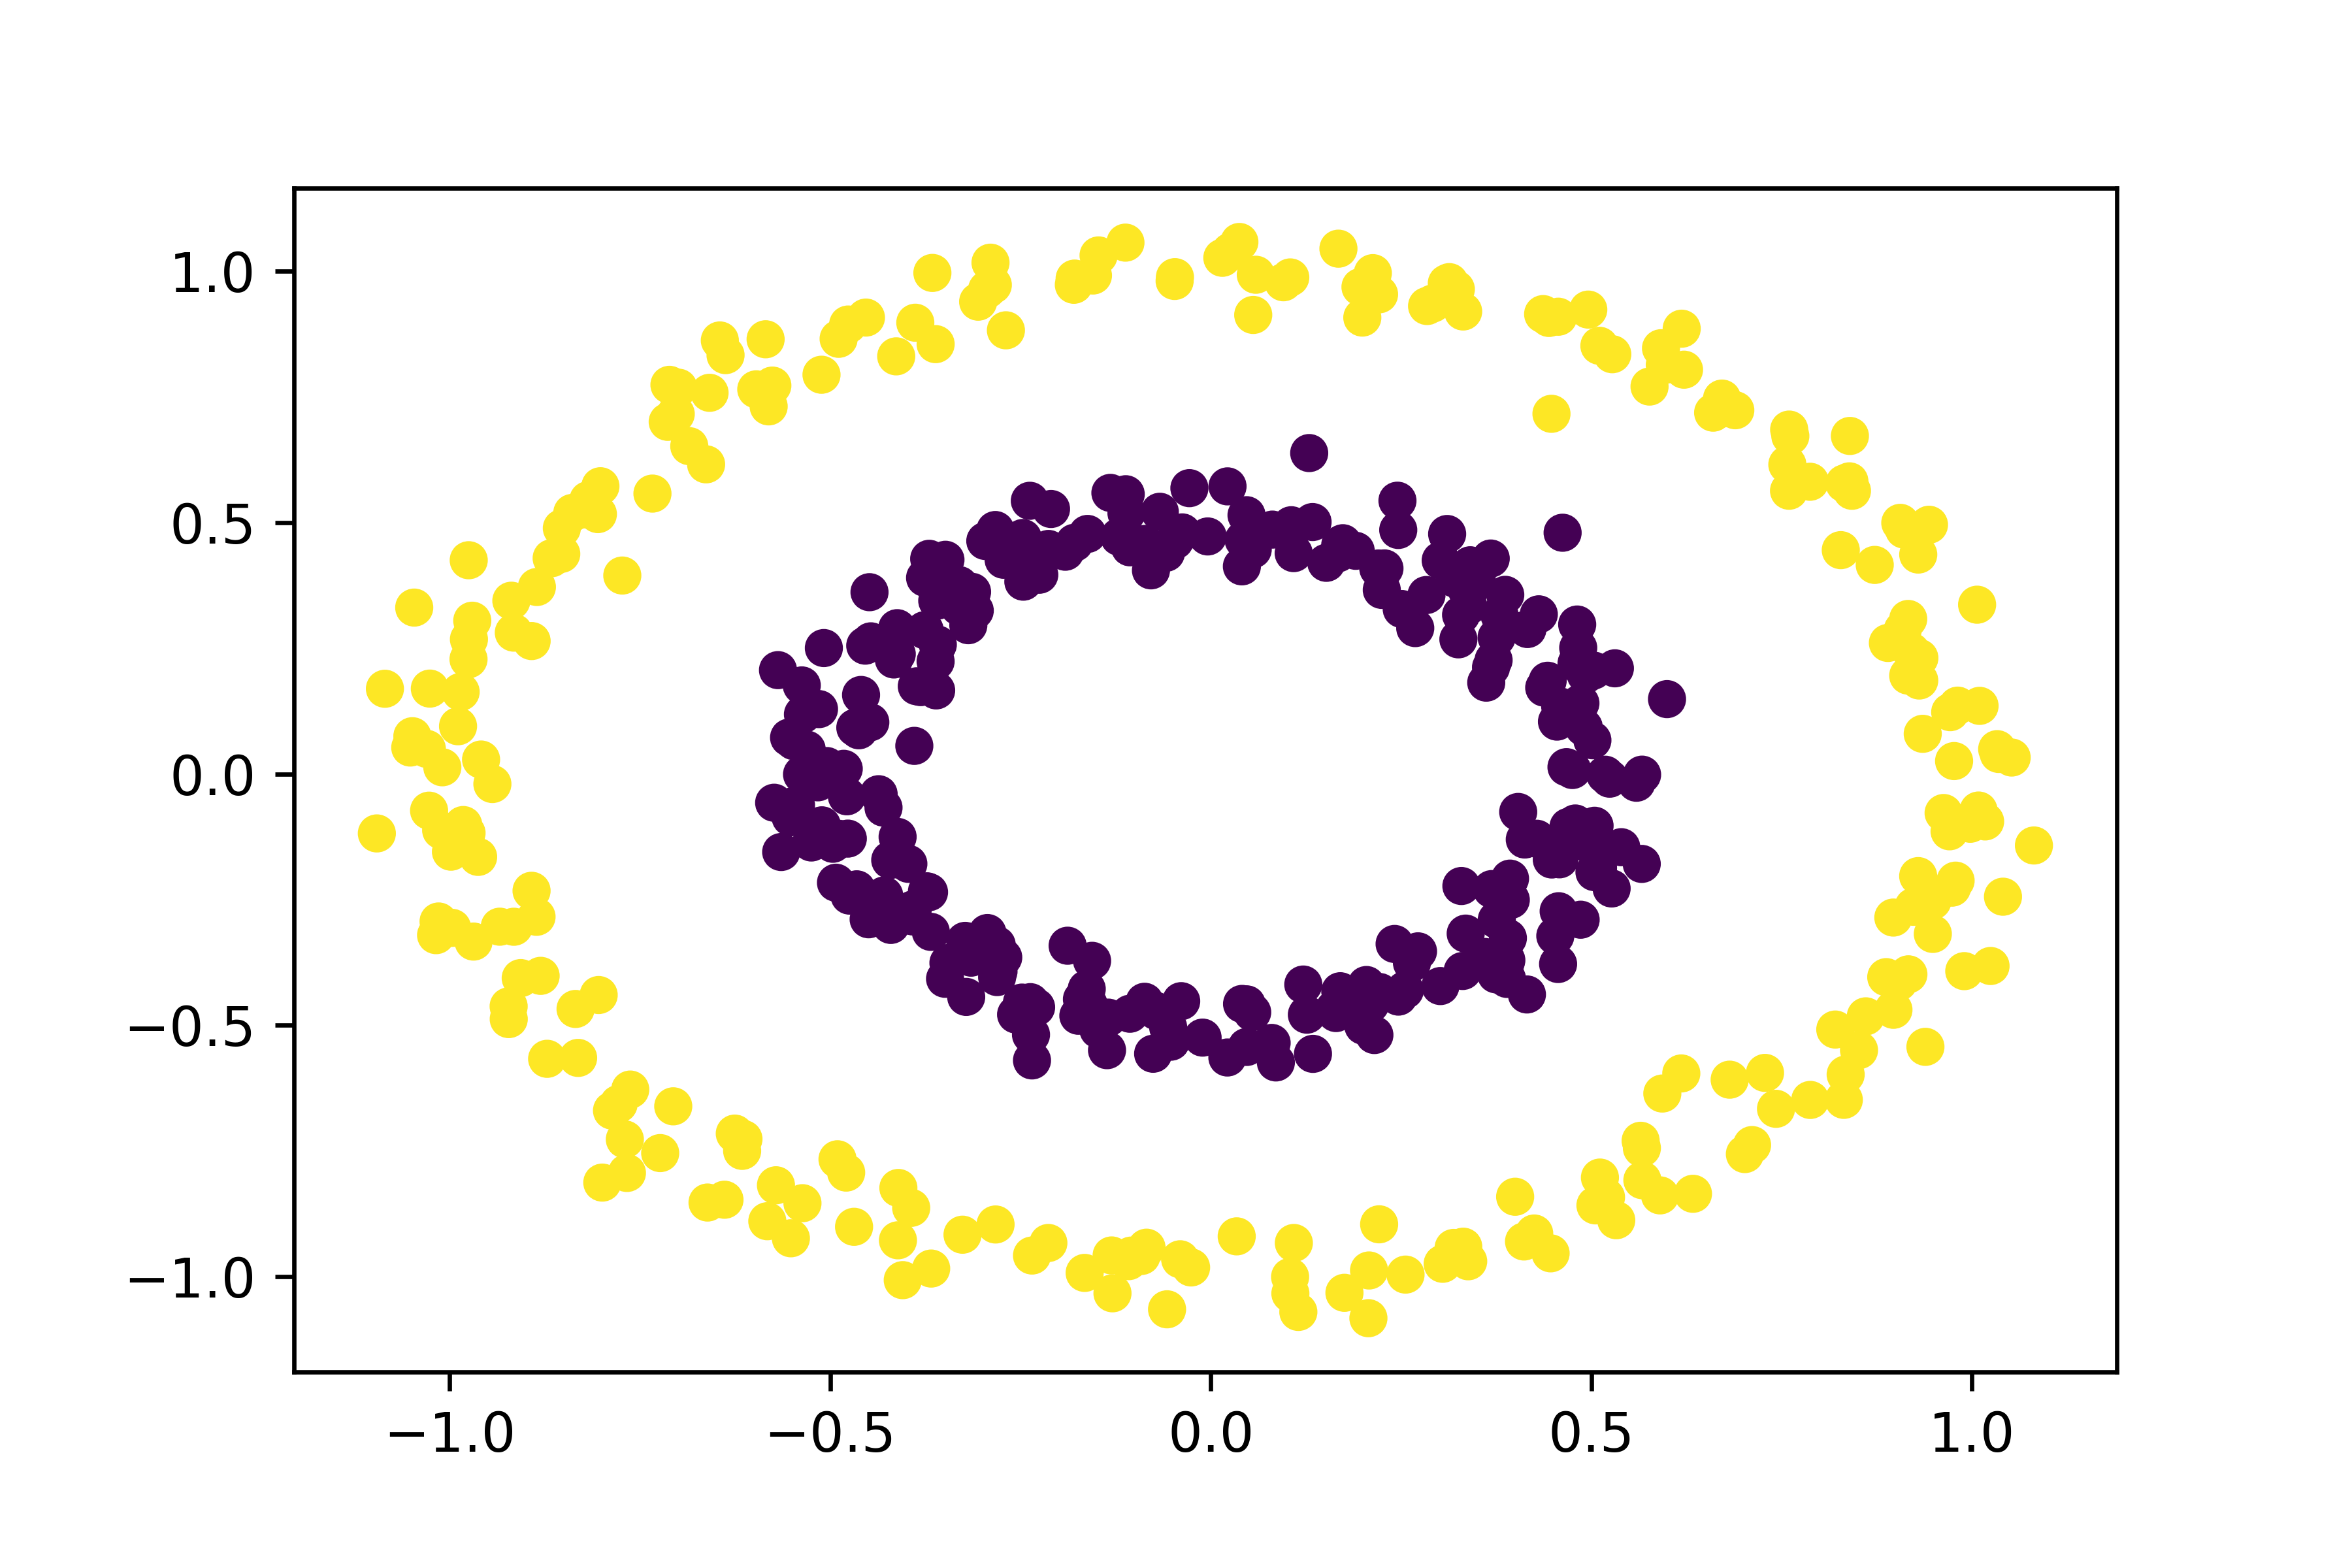
\includegraphics[width=1\linewidth]{kkm_53641.png}
        \caption{\textbf{SEED=53641}}
    \end{subfigure}%
    \begin{subfigure}{0.33\linewidth}
        \centering
        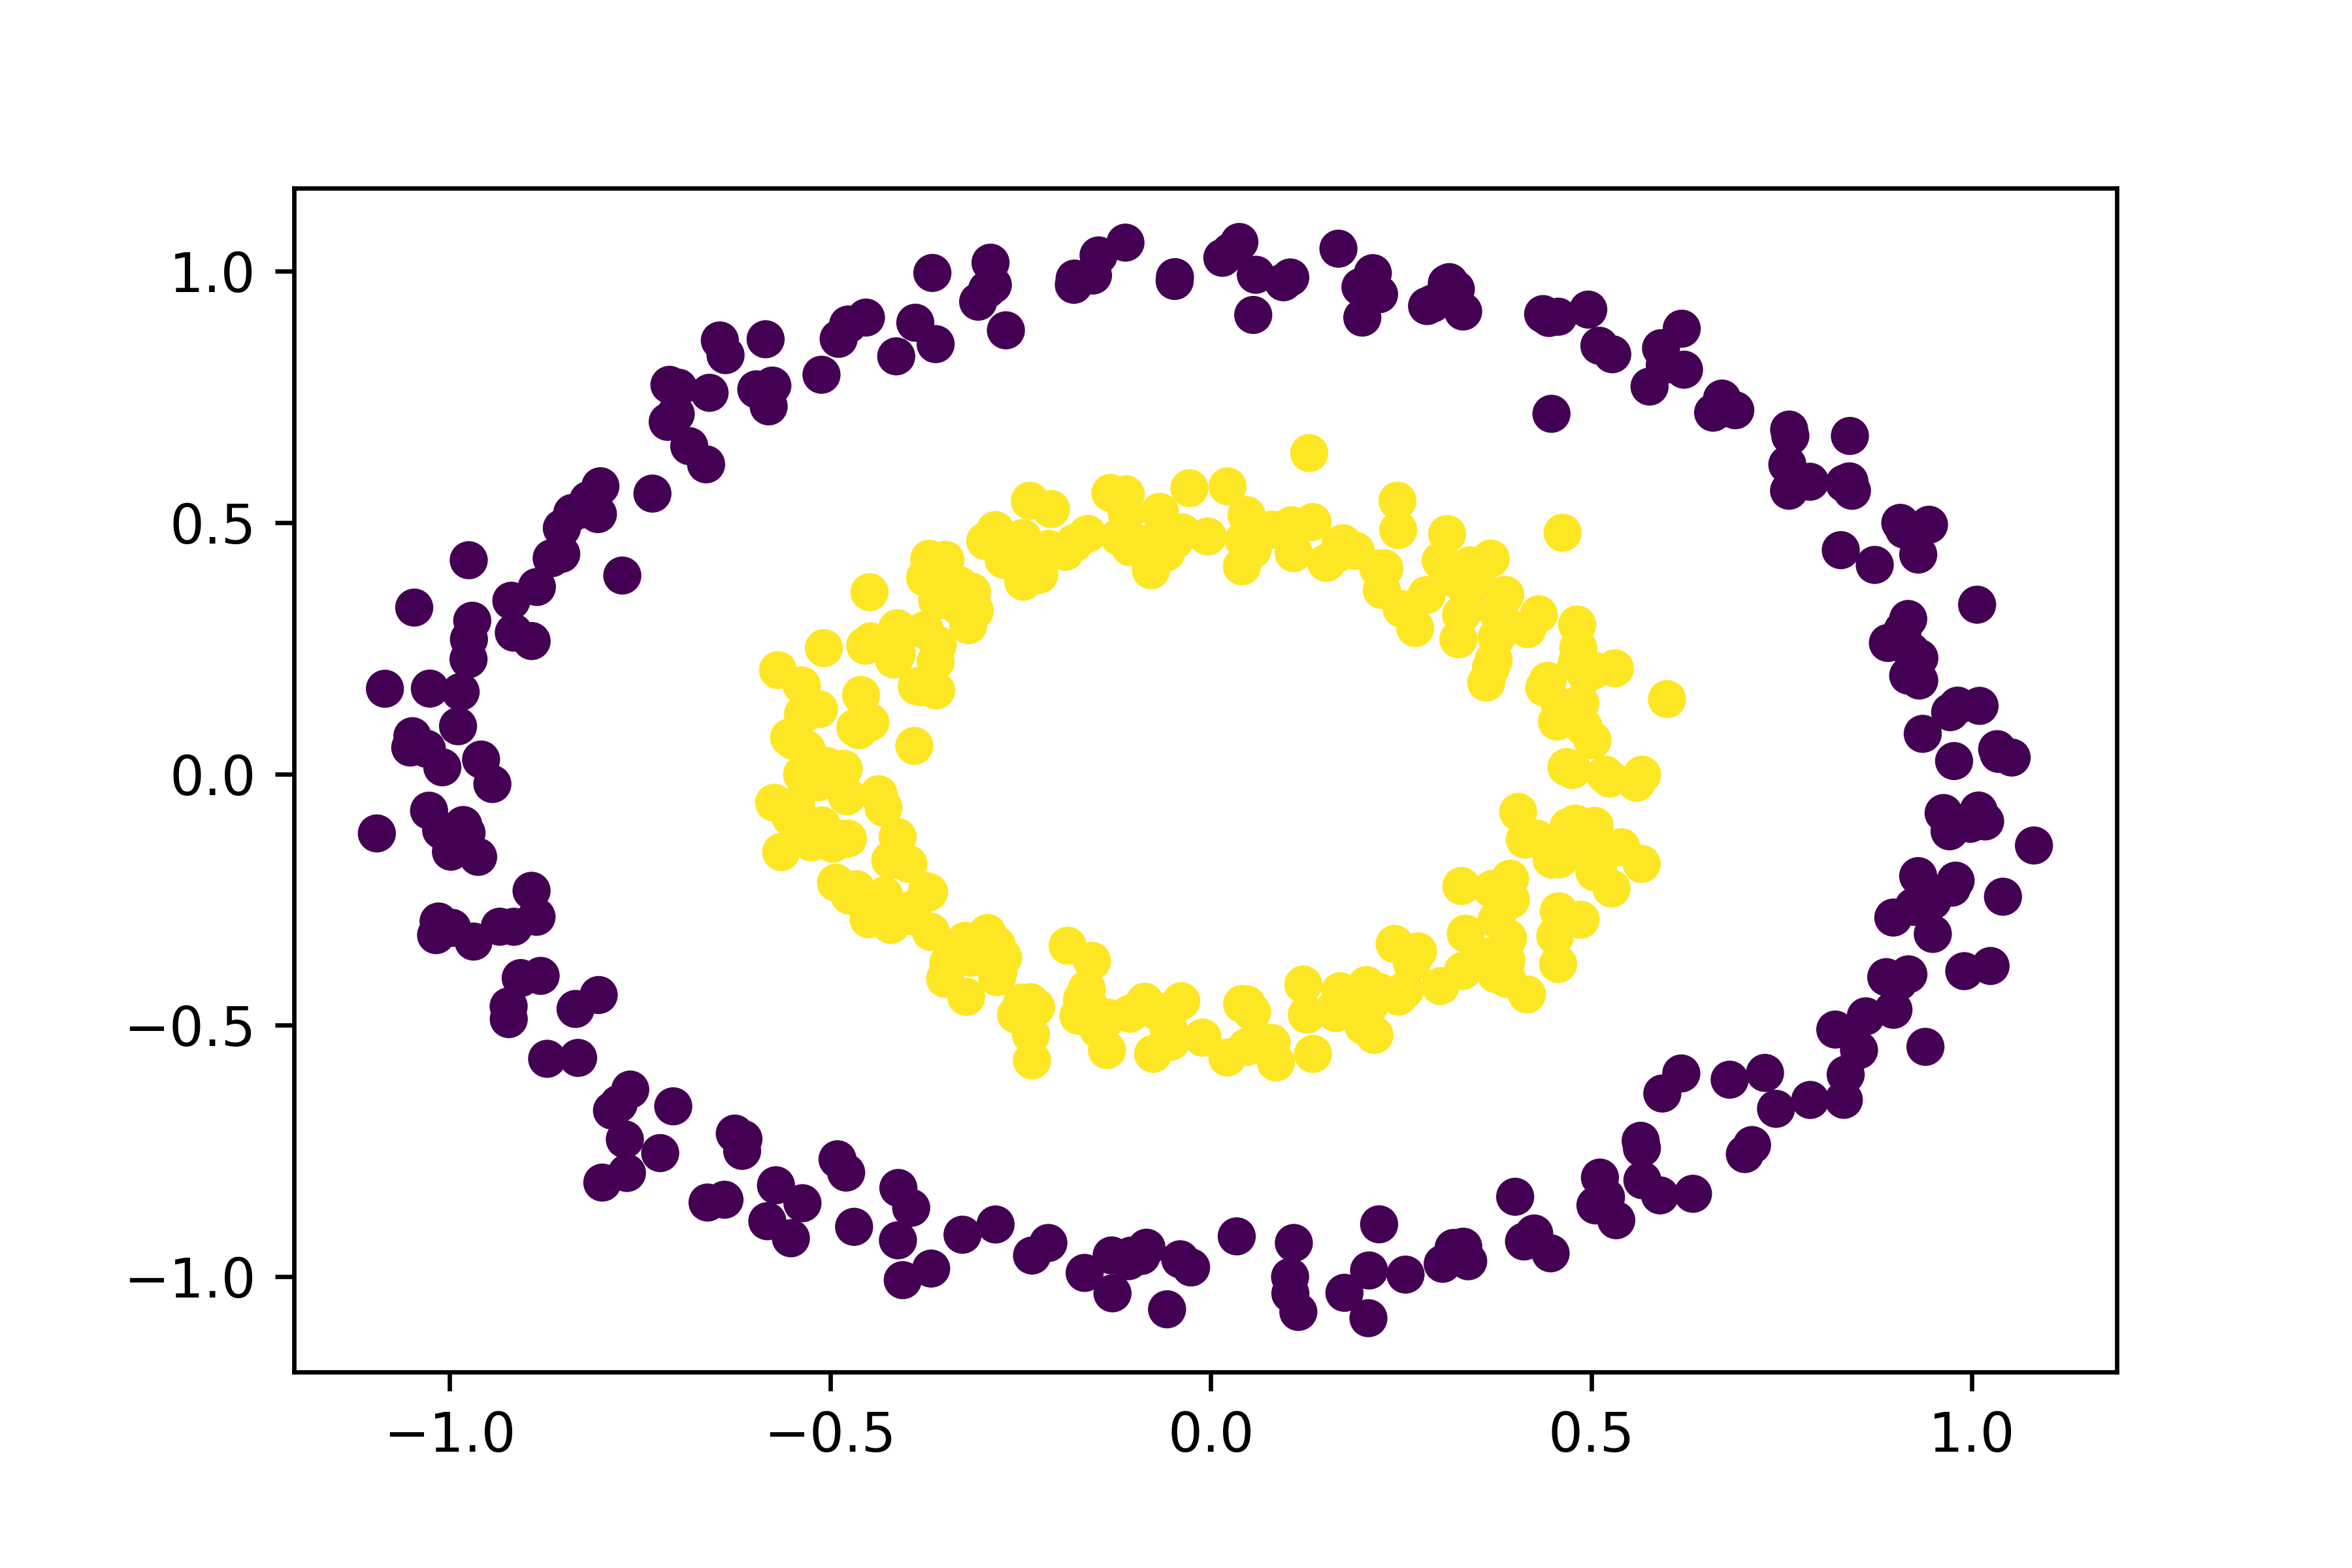
\includegraphics[width=1\linewidth]{kkm_87234.png}
        \caption{\textbf{SEED=87234}}
    \end{subfigure} 
    \caption{Kernel K-MEANS Clustered Dataset 3}   
\end{figure}

In the fit function we find and store the radius of the clusters as the $cluster\_centers$. In the predict function we calculate the squared distance between the cluster centers and norm of the data points. We allot the data point to the nearest cluster. 


\end{document}









